% !TeX encoding = UTF-8
% !TeX program = xelatex
% !TeX spellcheck = en_US

\documentclass[degree=master, language=english]{thuthesis}
  % 学位 degree:
  %   doctor | master | bachelor | postdoc
  % 学位类型 degree-type:
  %   academic(默认)| professional
  % 语言 language
  %   chinese(默认)| english
  % 字体库 fontset
  %   windows | mac | fandol | ubuntu
  % 建议终版使用 Windows 平台的字体编译


% 论文基本配置,加载宏包等全局配置
% !TeX root = ./thuthesis-example.tex

% 论文基本信息配置

\thusetup{
  %******************************
  % 注意:
  %   1. 配置里面不要出现空行
  %   2. 不需要的配置信息可以删除
  %   3. 建议先阅读文档中所有关于选项的说明
  %******************************
  %
  % 输出格式
  %   选择打印版(print)或用于提交的电子版(electronic),前者会插入空白页以便直接双面打印
  %
  output = print,
  %
  % 标题
  %   可使用“\\”命令手动控制换行
  %
  title  = {为躲避探测器的衣服生成自然纹理的扩散模型},
  title* = {Diffusion Models for Generating Natural-looking Textures for Clothes that Evade Detectors},
  %
  % 学科门类
  %   1. 学术型
  %      - 中文
  %        需注明所属的学科门类,例如:
  %        哲学、经济学、法学、教育学、文学、历史学、理学、工学、农学、医学、
  %        军事学、管理学、艺术学
  %      - 英文
  %        博士:Doctor of Philosophy
  %        硕士:
  %          哲学、文学、历史学、法学、教育学、艺术学门类,公共管理学科
  %          填写“Master of Arts“,其它填写“Master of Science”
  %   2. 专业型
  %      直接填写专业学位的名称,例如:
  %      教育博士、工程硕士等
  %      Doctor of Education, Master of Engineering
  %   3. 本科生不需要填写
  %
  degree-category  = {工学硕士},
  degree-category* = {Master of Science},
  %
  % 培养单位
  %   填写所属院系的全名
  %
  department = {计算机科学与技术系},
  %
  % 学科
  %   1. 研究生学术型学位,获得一级学科授权的学科填写一级学科名称,其他填写二级学科名称
  %   2. 本科生填写专业名称,第二学位论文需标注“(第二学位)”
  %
  discipline  = {计算机科学与技术},
  discipline* = {Computer Science and Technology},
  %
  % 专业领域
  %   1. 设置专业领域的专业学位类别,填写相应专业领域名称
  %   2. 2019 级及之前工程硕士学位论文,在 `engineering-field` 填写相应工程领域名称
  %   3. 其他专业学位类别的学位论文无需此信息
  %
  % professional-field  = {计算机技术},
  % professional-field* = {Computer Technology},
  %
  % 姓名
  %
  author  = {奚 墨},
  author* = {Bulatova Ekaterina},
  %
  % 指导教师
  %   中文姓名和职称之间以英文逗号“,”分开,下同
  %
  supervisor  = {胡 晓 林, 副教授},
  supervisor* = {Associate Professor Hu Xiaolin},
  %
  % 副指导教师
  %
  % associate-supervisor  = {陈文光, 教授},
  % associate-supervisor* = {Professor Chen Wenguang},
  %
  % 联合指导教师
  %
  % co-supervisor  = {某某某, 教授},
  % co-supervisor* = {Professor Mou Moumou},
  %
  % 日期
  %   使用 ISO 格式;默认为当前时间
  %
  % date = {2019-07-07},
  %
  % 是否在中文封面后的空白页生成书脊(默认 false)
  %
  include-spine = false,
  %
  % 密级和年限
  %   秘密, 机密, 绝密
  %
  % secret-level = {秘密},
  % secret-year  = {10},
  %
  % 博士后专有部分
  %
  % clc                = {分类号},
  % udc                = {UDC},
  % id                 = {编号},
  % discipline-level-1 = {计算机科学与技术},  % 流动站(一级学科)名称
  % discipline-level-2 = {系统结构},          % 专业(二级学科)名称
  % start-date         = {2011-07-01},        % 研究工作起始时间
}

% 载入所需的宏包

% 定理类环境宏包
\usepackage{amsthm}
% 也可以使用 ntheorem
% \usepackage[amsmath,thmmarks,hyperref]{ntheorem}

\thusetup{
  %
  % 数学字体
  % math-style = GB,  % GB | ISO | TeX
  math-font  = xits,  % stix | xits | libertinus
}

% 可以使用 nomencl 生成符号和缩略语说明
% \usepackage{nomencl}
% \makenomenclature

% 表格加脚注
\usepackage{threeparttable}

% 表格中支持跨行
\usepackage{multirow}

% 固定宽度的表格。
% \usepackage{tabularx}

% 跨页表格
\usepackage{longtable}

% 算法
\usepackage{algorithm}
\usepackage{algorithmic}

% 量和单位
\usepackage{siunitx}

% 参考文献使用 BibTeX + natbib 宏包
% 顺序编码制
\usepackage[sort]{natbib}
\bibliographystyle{thuthesis-numeric}

% 著者-出版年制
% \usepackage{natbib}
% \bibliographystyle{thuthesis-author-year}

% 本科生参考文献的著录格式
% \usepackage[sort]{natbib}
% \bibliographystyle{thuthesis-bachelor}

% 参考文献使用 BibLaTeX 宏包
% \usepackage[style=thuthesis-numeric]{biblatex}
% \usepackage[style=thuthesis-author-year]{biblatex}
% \usepackage[style=apa]{biblatex}
% \usepackage[style=mla-new]{biblatex}
% 声明 BibLaTeX 的数据库
% \addbibresource{ref/refs.bib}

% 定义所有的图片文件在 figures 子目录下
\graphicspath{{figures/}}

% 数学命令
\makeatletter
\newcommand\dif{%  % 微分符号
  \mathop{}\!%
  \ifthu@math@style@TeX
    d%
  \else
    \mathrm{d}%
  \fi
}
\makeatother

% hyperref 宏包在最后调用
\usepackage{hyperref}



\begin{document}

% 封面
\maketitle

% 学位论文指导小组、公开评阅人和答辩委员会名单
% 本科生不需要
% !TeX root = ../thuthesis-example.tex

\begin{committee}[name={学位论文指导小组、公开评阅人和答辩委员会名单}]

  \newcolumntype{C}[1]{@{}>{\centering\arraybackslash}p{#1}}

  \section*{指导小组名单}

  \begin{center}
    \begin{tabular}{C{3cm}C{3cm}C{9cm}@{}}
      胡晓林 & 副教授     & 清华大学 \\
      % 王XX & 副教授   & 清华大学 \\
      % 张XX & 助理教授 & 清华大学 \\
    \end{tabular}
  \end{center}


  \section*{公开评阅人名单}

  % \begin{center}
  %   \begin{tabular}{C{3cm}C{3cm}C{9cm}@{}}
  %     刘XX & 教授   & 清华大学                    \\
  %     陈XX & 副教授 & XXXX大学                    \\
  %     杨XX & 研究员 & 中国XXXX科学院XXXXXXX研究所 \\
  %   \end{tabular}
  % \end{center}


  \section*{答辩委员会名单}

  % \begin{center}
  %   \begin{tabular}{C{2.75cm}C{2.98cm}C{4.63cm}C{4.63cm}@{}}
  %     主席 & 赵XX                  & 教授                    & 清华大学       \\
  %     委员 & 刘XX                  & 教授                    & 清华大学       \\
  %         & \multirow{2}{*}{杨XX} & \multirow{2}{*}{研究员} & 中国XXXX科学院 \\
  %         &                       &                         & XXXXXXX研究所  \\
  %         & 黄XX                  & 教授                    & XXXX大学       \\
  %         & 周XX                  & 副教授                  & XXXX大学       \\
  %     秘书 & 吴XX                  & 助理研究员              & 清华大学       \\
  %   \end{tabular}
  % \end{center}

\end{committee}



% 也可以导入 Word 版转的 PDF 文件
% \begin{committee}[file=figures/committee.pdf]
% \end{committee}


% 使用授权的说明
\copyrightpage
% 将签字扫描后授权文件 scan-copyright.pdf 替换原始页面
% \copyrightpage[file=scan-copyright.pdf]

\frontmatter
% !TeX root = ../thuthesis-example.tex

% 中英文摘要和关键字

\begin{abstract}
   (TODO: autotranslated) 最近,在构建物理上可实现的探测器规避攻击方面取得了巨大成功。
   尽管该领域取得了快速进展,但物理领域的对抗性攻击仍然常常不切实际:人眼很容易发现对抗性示例,因为它们不寻常的鲜艳颜色或过于显眼的怪异图案。
  
   在这篇硕士论文中,我们提出了一种方法来创建真实的对抗纹理以逃避检测器,但在性能方面仍可与最先进的检测器竞争。
   受扩散概率模型强大生成能力的启发,我们采用预训练模型,通过指导生成物理上可实现的服装对抗纹理。
  
   论文通过将结果与基线方法进行比较,证明了所提出的方法生成的模式的有效性、自然性和可控性。
   虽然模式的对抗效应并不高于最先进的方法,但我们的策略可以控制模式并能够以自然性来交换对抗效应。
   此外,由于该方法适用于预训练模型,因此它比基线要快得多。

  % 关键词用“英文逗号”分隔,输出时会自动处理为正确的分隔符
  \thusetup{
    keywords = {对抗性攻击、物体识别、扩散模型、物理攻击、指导},
  }
\end{abstract}

\begin{abstract*}
  Recently, huge success has been achieved in constructing physically realizable evasion attacks on detectors.
  Despite the rapid progress in the area, adversarial attacks in the physical domain still often suffer from being unrealistic: the human eye can easily spot adversarial examples due to their unusual vivid colors or overly conspicuous bizarre patterns.
  
  In this master thesis, we propose a method to create realistic adversarial textures for evading detectors that would nevertheless compete with the state-of-the-art ones in terms of performance.
  Motivated by the strong generation abilities of diffusion probabilistic models, we employ pretrained models for generation of physically realizable adversarial texture for clothing using guidance.
  
  The thesis demonstrates the effectiveness, the naturalness, and the controlability of the patterns generated with the proposed method by comparing the results against baseline methods.
  While the adversarial effect of the patterns is not higher than that of the state-of-the-art methods, our strategy gives control over the pattern and enable trading adversarial effects off for naturalness.
  Moreover, since the method works on pretrained models, it is significantly faster than the baselines.

  % Use comma as separator when inputting
  \thusetup{
    keywords* = {adversarial attacks, object detection, diffusion models, physical attacks, guidance},
  }
\end{abstract*}


% 目录
\tableofcontents

% 插图和附表清单
% 本科生的插图索引和表格索引需要移至正文之后、参考文献前
% \listoffiguresandtables  % 插图和附表清单(仅限研究生)
\listoffigures           % 插图清单
\listoftables            % 附表清单

% 符号对照表
% !TeX root = ../thuthesis-example.tex

\begin{denotation}[3cm]
  \item[AP] Average Precision
  \item[ASR] Attack Success Rate
  \item[bbox] Bounding BOX
  \item[CLIP] Contrastive Language-Image Pre-training
  \item[CNN] Convolutional Neural Network
  \item[COCO] Common Objects in COntext, Microsoft dataset for object detection 
  \item[CV] Computer Vision
  \item[DETR] DEtection TRansformer, a transformer-based object detection model 
  \item[DL] Deep Learning
  \item[DM] Diffusion Model
  \item[DNN] Deep Neural Network
  \item[IoU] Intersection over Union
  \item[LM] Language Model
  \item[ML] Machine Learning
  \item[R-CNN] Regions with CNNs, a region-based object detection model 
  \item[RL] Reinforcement Learning
  \item[TPS] Thin plate splines, augmentation technique for imitating clothes
  \item[VAE] VAriational Encoder
  \item[YOLO] You Only Look Once, a grid-based object detection model 
\end{denotation}



% 也可以使用 nomencl 宏包,需要在导言区
% \usepackage{nomencl}
% \makenomenclature

% 在这里输出符号说明
% \printnomenclature[3cm]

% 在正文中的任意为都可以标题
% \nomenclature{PI}{聚酰亚胺}
% \nomenclature{MPI}{聚酰亚胺模型化合物,N-苯基邻苯酰亚胺}
% \nomenclature{PBI}{聚苯并咪唑}
% \nomenclature{MPBI}{聚苯并咪唑模型化合物,N-苯基苯并咪唑}
% \nomenclature{PY}{聚吡咙}
% \nomenclature{PMDA-BDA}{均苯四酸二酐与联苯四胺合成的聚吡咙薄膜}
% \nomenclature{MPY}{聚吡咙模型化合物}
% \nomenclature{As-PPT}{聚苯基不对称三嗪}
% \nomenclature{MAsPPT}{聚苯基不对称三嗪单模型化合物,3,5,6-三苯基-1,2,4-三嗪}
% \nomenclature{DMAsPPT}{聚苯基不对称三嗪双模型化合物(水解实验模型化合物)}
% \nomenclature{S-PPT}{聚苯基对称三嗪}
% \nomenclature{MSPPT}{聚苯基对称三嗪模型化合物,2,4,6-三苯基-1,3,5-三嗪}
% \nomenclature{PPQ}{聚苯基喹噁啉}
% \nomenclature{MPPQ}{聚苯基喹噁啉模型化合物,3,4-二苯基苯并二嗪}
% \nomenclature{HMPI}{聚酰亚胺模型化合物的质子化产物}
% \nomenclature{HMPY}{聚吡咙模型化合物的质子化产物}
% \nomenclature{HMPBI}{聚苯并咪唑模型化合物的质子化产物}
% \nomenclature{HMAsPPT}{聚苯基不对称三嗪模型化合物的质子化产物}
% \nomenclature{HMSPPT}{聚苯基对称三嗪模型化合物的质子化产物}
% \nomenclature{HMPPQ}{聚苯基喹噁啉模型化合物的质子化产物}
% \nomenclature{PDT}{热分解温度}
% \nomenclature{HPLC}{高效液相色谱(High Performance Liquid Chromatography)}
% \nomenclature{HPCE}{高效毛细管电泳色谱(High Performance Capillary lectrophoresis)}
% \nomenclature{LC-MS}{液相色谱-质谱联用(Liquid chromatography-Mass Spectrum)}
% \nomenclature{TIC}{总离子浓度(Total Ion Content)}
% \nomenclature{\textit{ab initio}}{基于第一原理的量子化学计算方法,常称从头算法}
% \nomenclature{DFT}{密度泛函理论(Density Functional Theory)}
% \nomenclature{$E_a$}{化学反应的活化能(Activation Energy)}
% \nomenclature{ZPE}{零点振动能(Zero Vibration Energy)}
% \nomenclature{PES}{势能面(Potential Energy Surface)}
% \nomenclature{TS}{过渡态(Transition State)}
% \nomenclature{TST}{过渡态理论(Transition State Theory)}
% \nomenclature{$\increment G^\neq$}{活化自由能(Activation Free Energy)}
% \nomenclature{$\kappa$}{传输系数(Transmission Coefficient)}
% \nomenclature{IRC}{内禀反应坐标(Intrinsic Reaction Coordinates)}
% \nomenclature{$\nu_i$}{虚频(Imaginary Frequency)}
% \nomenclature{ONIOM}{分层算法(Our own N-layered Integrated molecular Orbital and molecular Mechanics)}
% \nomenclature{SCF}{自洽场(Self-Consistent Field)}
% \nomenclature{SCRF}{自洽反应场(Self-Consistent Reaction Field)}



% 正文部分
\mainmatter
% !TeX root = ../thuthesis-example.tex

\chapter{INTRODUCTION}

Deep Neural Networks (DNNs), an architecture of the large family of Deep Learning (DL) algorithms, are a powerful tool that is nowadays used for solving countless practical challenges.

In fact, almost every part of our everyday lives can be automatized to a certain degree with the help of an appropriate tool build upon a DNN.
Cars and other vehicles can rely on Computer Vision (CV) systems for autonomous driving; the problem of international communication between people who do not know foreign languages had been significantly alleviated with the help of translation provided by Language Models (LMs); data analysis with the use of various basic Machine Learning (ML) techniques can now produce more accurate predictions for future trends in such important fields as finances, medicine, natural disaster prevention, and others; Reinforcement Learning (RL) enabled improvements in robotics, and so on.

A major problem that surfaces as the trend to deploying DNNs in all fields of our lives continues to gain momentum is the reliability of the said systems.
In particular, even though the DNNs work exceptionally well on many tasks, they are known to be fragile to adversarial examples: an attacker can perturb input data in a way that the predictions of the model will be damaged.

This thesis addresses the aforementioned problem by demonstrating a way to construct such malicious examples. 
Thus, the work lies at the intersection of three major areas of DL: detection, adversarial attacks, and diffusion models.
In this section, we delve a little deeper into these three areas as we introduce their importance to our modern fast-paced world.

% TODO more here: I need like 2+ pages

\section{Detection}

CV tasks are one of the largest areas of research in DL.
The human eye and brain are capable of acquiring and processing visual information easily and in an instant.
By looking at a single picture, we immediately gain overall understanding of the situation, simultaneously retrieving a lot more data than we even realize. 

In modern CV systems, however, the tasks are typically solved separately by applying different DL systems.
For example, just as we can immediately ``name'' a picture by analyzing the overall content and thus successfully categorizing the given image, a classification model can label images according to the classes that were introduced to the model during the training process.
This particular task is called image classification, and, as far as the architectures of such models go, the task is relatively simple: in some cases, a single CNN (Convolutional Neural Network) that outputs probabilities of the classes for each given input is enough to achieve decent results.

Image classification, however, is far from being the only task in the large research area that CV is.
Let us turn our attention to another ability our human vision provides: ability to detect and recognize various objects.
Imagine driving down the street in a busy city.
As a driver, you have to constantly monitor the situation outside your car windows: you have to quickly note and recognize road signs, watch over pedestrians that may want to cross the street, carefully keep your distance from other cars---after all, to err is human, and any driver must be ready to make swift decisions in response to other people's mistakes such as unskillful driving or crossing road in undesignated areas.
For us, as for researchers of the CV area, this task is called object detection.
If we describe the problem in a slightly more formal manner, it will sound like this: given an input image, our system is required to find all relevant to our task objects and classify them.
Thus, the output of our system will more likely consist of three parts: firstly, the coordinates for every found object, secondly, what classes the objects are, and lastly, how confident the model is in these predictions.
The last part is also easy to understand if you imagine being a driver that looks through a dirty window of their car trying to understand if the silhouette on the road in front of them is an animal or just a pool of water.
If the driver is sufficiently confident that this is nothing but a pool, they can continue driving normally; otherwise, they need to stop the car.

Normally, unlike in a similar task of image segmentation where we have to provide class for each pixel of our input image, in case of object detection, we are only asked to provide a bounding box (bbox) around each object.

A large number of models with DNN backbones has been proposed to solve the object detection challenge, and the state-of-the-art methods in this field and have achieved high detection accuracy. 
For instance, the most famous works in this area include Faster R-CNN~\cite{faster_rcnn} (Faster Regions With CNNs), DETR~\cite{detr} (Detection Transformer), and YOLO~\cite{yolov3} end-to-end detectors.

% TODO more...

\section{Adversarial Attacks}

As we have previously established, the fact that the DNNs are gradually getting into so many areas of our lives, gives rise to major concerns with the reliability of the DNNs.

Despite the exceptional results the DNNs show in most if not all of their applications, they have been proven to not be stable and consistent in their predictions, which can be exploited with malicious intents.
The adverse effects of adversarial attacks are attracting a lot of attention now in light of the sheer amount of models produced for fault-sensitive practical tasks nowadays, such as detection modules of self-driving cars, chatbots, medicine, facial recognition systems and other applications, where a single mistake can cost lots of money or even human lives.

Unlike a DNN that is sensitive from the out-of-distribution input data to its inside architecture and training parts such as hyperparameters or initialization, the human eye is hard to fool.
For example, let us consider the aforementioned task of image classification.
When we see an image of a cat, we can immediately categorize it as such, even if the photo is perhaps a little bit dirty or even missing some parts.
For a fragile CV system, however, a slight perturbation in the input data may be enough to give out completely incorrect prediction, going as far as to become absolutely sure that the provided image depicts a car, while for the human eye, the same perturbation will go undetected.
It is easy to imagine an attacker changing a small set of pixels or adding unnoticeable noise to an input image; yet CV is not the only area vulnerable to such attacks. 
Even LMs that might seem more stable are susceptible to them: additional lines attached to the ending of an input line, or even seemingly unimportant and harmless typographical errors in given data may lead to abnormal behaviour of LMs. 
In recent years, many adversarial examples on different kinds of DNNs have been constructed, such as~\cite{first_adv, fgsm, pgd} etc.

In our case, however, as it has been mentioned previously, we are concerned with the safety a very specific area of DL: object detection.
Attack on detection models are normally not as easy as attacks on less convoluted CV models like classifiers, yet it was shown that they are entirely plausible.
Again, by introducing inconspicuous to the human eye changes to input data, one can cause the detectors to behave in bizarre ways.
As we have established, a typical detection system output consists of three parts: bboxes that denote the position of elements, classes for each of them, and the confidence in found objects.
Naturally, adversarial samples may aim to impair the operation of the detector with different corresponding attack types.
For example, if an attack only causes the model to assign an incorrect class, while still finding bboxes, this attack will be called a \textit{misclassification} attack.
As the title of the thesis shows, however, we are interested in avoiding detection altogether by performing \textit{evasion} attacks.
In practice, these attacks aim to lower the confidence of the detected bboxes.
Let us imagine for a moment that we have come up with some kind of ``perfect'' evasion adversarial attack and our victim object detection model stopped detecting any objects of our interest, say, people.
Now lets also assume that the victim detection model is actually a part of a CV system that dictates the movements to a car set on autonomous driving.
Since the system is no longer able to detect humans at all, it will completely ignore any pedestrians, which will result in a car accident.
Thus, it is easy to understand just how important it is to ensure the safety of our CV systems and protect them against adversarial attacks.

Given the importance of the stability of object detection systems, there is no wonder that the area does not lack active research.
However, most of the attacks focus on achieving a higher attack success rate (ASR) and give little attention to how natural their adversarial perturbations seem to humans.
Yet the lack of naturalness in adversarial examples lowers the value of the attack since such samples draw unwanted attention from human observers; moreover, it is easier to protect a CV system from such unnatural patterns than against those that seem harmless.
Again, in practice, natural adversarial examples are important since they might be used for threatening models that absolutely need to be robust, like detectors in self-driving cars.

Furthermore, when it comes to practical applications in CV tasks, we become rather interested in physical scenarios instead of the digital ones.
After all, the attacker rarely has access to the insides of a CV system, while changing the physical world by, for example, attaching a sticker to a road sign, is possible for everyone.
While for the attacks in the digital space, it is fairly easy to introduce an inconspicuous change to the input data to fool the human eye, most of the physical attacks look unnatural since the task itself is way more difficult and requires more robust solutions compared to those in the digital space.
In their turn, the adversarial samples also need to be way more robust than their digital analogies.

To address this issue, many natural-looking physical attacks have been introduced~\cite{stop_signs_detectors_380, dog_patch_clothes, wang2021dual}.
For the detection task, the adversarial attacks are mainly created as patches and stickers~\cite{spatial_context, aerial_patch, rp2} or textures~\cite{car_camo, texture}.

Stickers and patches are small pieces of paper with adversarial patterns, that can be attached to something in the real world and disrupt the behaviour of their victim CV systems.
Textures, in this case, are something that ``envelopes'' an entire object, like clothes to a person or colored surfaces to cars.

For the physical scenario, textures are preferable since a patch only retains its adversarial qualities at a limited range of angles of the camera in the real world.
While it is possible to attach adversarial patches all over the object to avoid this problem at least partially, an object that has the same non-pattern patch repeated all over itself will look unnatural, while a texture would not attract as much attention.
There are, of course, certain limitations to textures, even compared to patches.
For instance, only a very limited range of objects does not look strange covered in a texture; normally, only personal belongings like clothes or car patterns that have been already mentioned before do not look suspicious when heavily personalized, unlike public objects like roads or signs.
Patches, however, suffer from a similar problem since any foreign objects attached to things in public spaces are considered trash and removed as soon as the human eyes spots them.

While adversarial attacks by themselves have a negative societal impact in the sense that they might be used to fool DNNs with malicious purposes, we believe that this research can help with defending against attacks like this.
Just like in cybersecurity where the people work either in the blue team coming up with defense techniques or in the red designing methods for attacks, we aim to push forward research that focuses on making the CV systems in all their forms more secure and robust.

% TODO more...

\section{Diffusion Models}

Another research area that is highly relevant to this thesis is generative artificial intelligence, in particular, image generation in CV.

The first thought that comes to mind when it comes to applications of image generation is its artistic value, yet the usage of generative models go way beyond this.
For this research, it is important to understand that they can play a big role in producing adversarial samples.
For example, a correctly trained model can generate malicious out-of-distribution examples. 
While it is extremely useful in terms of how they can be used like augmentations to complement existing datasets for training more stable models, the models can also be used for attacking various systems.

For example, the patches, stickers, and textures we have discussed in the previous section can not only be constructed by perturbing existing patterns, but created from noise with generative models.

IN particular, we are interested in generative abilities of diffusion models (DMs).
DMs performed excellently on many tasks, and using them for generating adversarial samples is a relatively novel and promising way since overall DMs remain an underexplored research area even today.

A DM is usually given a text prompt as input and is required to produce a corresponding image.
Overall, without going to deep into detail in the introduction part, while generating samples, pretrained DMs gradually remove noise from a random import, overall moving into the direction conditioned by the given prompt.
Since the process is gradual and consists of many steps, one can alter the direction by bringing change to this trajectory.
This particular property of DMs that is called \textit{guidance} is important in this research since it means that there might be a way to alter that direction of a pretrained model to make it produce adversarial sample without even any additional training.

% TODO more!!

\section{Thesis Goal}

Now, armed with at least superficial understanding of all areas that are related to the research in this thesis, we can finally formulate the goal we are pursuing.

In short, we are to find a way to create physically realizable adversarial textures that are not immediately recognized as a threat by the human eye.
The created framework should help to obtain such realistic adversarial textures for suppression of predictions of a detector by generating them with a diffusion model.

That is, we want to be able to generate patterns for clothes that make a person invisible to victim object detectors.

The created texture is to satisfy to three requirements: it has to be \textit{effective}, \textit{natural}, and \textit{controllable}.

% TODO include the examples from other papers as sota

\begin{itemize}
    \item \textit{Effective} means that our clothes should hide the attacker from all angles, not like a patch that only works from a certain angle.

    \item \textit{Natural} means that the clothes should not look suspicious to the human eye. 
    That requirement prohibits us from simply generating an adversarial image and tiling the entire clothes with it since a repetition of a random image looks highly unnatural.

    \item \textit{Controllable} means that we want to be able to generate a wide range of patterns depending on what the user (in our case---attacker) wants to see.
    This requirement is important because, as we will see in the literature review section, there are few methods that provide an opportunity to control the generated adversarial pattern in the physical world.
\end{itemize}

\section{Contribution}

The pipeline proposed in this thesis satisfies the requirements defined above.
The newly introduced method has the following main advantages:

\begin{itemize}
    \item \textbf{Effectiveness and naturalness}.
    While this method does not beat the state-of-the-art ones in terms of how well the adversarial textures hide people from detection, this method allows to trade the adversarial effectiveness for achieving additional naturalness.
    \item \textbf{Speed}.
    Due to the fact that that we only use pretrained models, the method is significantly faster than other methods that require additional training.
\end{itemize}

% TODO more




% !TeX root = ../thuthesis-example.tex

\chapter{Literature Review}

In this section, we will provide a broad overview of the existing methods and the references that motivated the project.

\section{Digital adversarial examples}
The first ones to discover adversarial examples were the authors of~\cite{first_adv} who used gradients of the model to construct an imperceptible to the human eye noise that changed the prediction of the DNN.

Formally, a perturbation $\delta$ for a DNN $f$ is adversarial if $f(x+\delta) \ne f(x)$ and $\delta$ meets certain requirements; most commonly, we aim to minimize $\delta$ and look for a perturbation in a certain radius $\epsilon$ with respect to norm $L_{p}$: $||\delta||_p < \epsilon$.
In this case, $x + \delta$ is called an adversarial example.

After the initial discovery in~\cite{first_adv}, such adversarial examples have quickly gained popularity and have been studied in many areas and applications.

Over the years, many attacks have been created for all kinds of scenarios.
The authors of~\cite{first_adv} simply attacked a classifier by finding a small perturbation that causes a misclassification via minimizing the loss between the perturbed image and the target class.
This method is called the L-BFGS Attack.
Soon after, more advanced methods such as the popular Fast Gradient Sign Method (FGSM) from~\cite{fgsm} that produces adversarial examples by moving against the gradients or the Projected Gradient Descent (PGD) attack from~\cite{pgd} that is basically an improved projected iterative version of FGSM.
The DeepFool algorithm from~\cite{deepfool} looks for an adversarial example with the smallest perturbation, and the Jacobian-based Saliency Map Attack (JSMA) from~\cite{jsma} finds the most influential pixels and changes their values to either maximum or minimum.
~\cite{carlini_attacks} improved the L-BFGS method by switching to logits in loss and changing variables, the FGSM attack by a softer penalizing, and the JSMA method by shrinking the set of changeable pixels instead of growing it.

These attacks suggest that the attacker can get the gradients of the victim model and are called white-box attacks.
This suggestion, however, does not necessarily hold true, as in a real life scenario, the attacker is rarely given access to the model.
If the attacker can not get the gradients, they have to use different approaches; such scenarios are called black-box attacks. 
Many methods were developed for this case as well.
Ones of the first famous works in this field include~\cite{probably_first_bb} and~\cite{famous_bb} who studied adversarial sample transferability.


DNNs turned out to be so vulnerable to adversarial attacks that changing even one pixel might be enough to fool them~\cite{one_pixel}.
\cite{universal} explored a way to create a small perturbation vector that is able to fool the classifier for any input image. 
~\cite{classifier_patch, classifier_patch2} created patches: localized adversarial noise that only covers a limited number of pixels concentrated in one area.
Improvements to existing methods have been introduced, like the momentum-based iterative algorithm from~\cite{adv_momentum} that boosts adversarial attacks, the translation-invariant attack method from~\cite{adv_translation_invariant} or Adam Iterative Fast Gradient Method from in~\cite{adv_optimizer} that improve the transferability between models, which is especially useful for the black-box scenarios.

Another classification of the attack according to their aims is the targeted versus untargeted classification.
Untargeted attacks, like the classical versions of FGSM, PGD and L-BFGS, simply aim to thwart the predictions of the models in any way, while the targeted attacks aim to force the model to behave in a particular way.
Normally, in order to create a targeted attack, one has to force the predictions to move towards the needed result instead of moving away from the true prediction, so instead of maximizing loss, one has to minimize it in a specific direction.

\section{Physical attacks on detectors}
In this work, we are mainly concerned with adversarial attacks on detectors.
The final output of a detector consists of a bounding box, a confidence score and a class for every predicted object.
By choosing different loss functions, an attacker can construct many attacks that aim at interfering with different output values of a detector.
Mainly, there are two types of attacks on detectors: the ones that cause misclassification of boxes, like~\cite{det_misclas}, and the ones that suppress predictions, like~\cite{physical_patch}.
The adversarial examples that trigger misclassification were likely with a loss function that disturbed the classification loss of the detector, while the suppression attacks use losses that try to lower the confidence score of the predicted boxes.

There are also different ways to attack detectors depending on how an attacker constructs their adversarial structure.
The most commonly used ones are adversarial patches and adversarial textures.
In some cases, optical attacks are used as well.
For this, an attacker has to change lighting or perform the attack with lasers. 
Even though such attacks are stealthy, they are hard to utilize in practice since they are susceptible to environmental light.

Interestingly, since detector make their predictions partially based on the background, as shown in such papers as~\cite{det_context_emp_study, dec_context_evaluation, det_context_attentive}, there is a way to create an adversarial object that would suppress not only the closest boxes that overlap with the object, but also other predictions that might be far away from it.
The authors of~\cite{dpatch} claimed to have created a patch that can suppress all predictions on an input image.
These results are, however, non reproducible since the authors have made several fatal mistakes such as not clipping their patch to the real color range and not freezing all the weights of the detector while training the patch.
Other papers, however, corrected the errors and produced more realistic results.
The authors of~\cite{physical_patch} went a step further and trained their patch with augmentations that allowed printing the patch and thus affecting a detector in the physical world.
In order to produce such realistic augmentations, the authors applied the Expectations over Transformations approach from~\cite{eot}.
Unlike~\cite{dpatch}, who were mainly concerned with targeted attacks in a sense that they forced all predictions of the model leave their original positions to concentrate around the patch, the~\cite{physical_patch} created an untargeted attack that instead aims to hide as many objects as possible.
Their patch is, however, pretty large as its side takes one fourth of the screen; moreover, as we have mentioned before, it neither takes into account the naturalness of its appearance nor retains its adversarial qualities when the camera angle shifts, unlike adversarial textures.
Similarly, the authors of~\cite{patch_conf_pgd} perform a PGD attack on the confidence scores to hide all objects and produce real-life adversarial examples.
They tried out different configurations and performed an ablation study that suggests that the classification loss, that was also used in~\cite{physical_patch}, does not improve the patch.

Some other approaches aim to hide or suppress only a certain range of predictions.
For example, the authors of~\cite{spatial_context} create a patch that makes the detector blind to all, even non-overlapping, objects of a certain class.
Similarly,~\cite{aerial_patch} create an adversarial patch that hides vehicles from automatic detectors.

A wide range of works is aimed at perturbing stop signs since they are crucial for self-driving cars \cite{signs_digital, stop_signs_detectors_380, sign_shapeshifter, sign_2020_16, signs_shadows}.
Among them,~\cite{signs_shadows} is an optical attack: the attacker casts a shadow over a road sign to distort the predictions of the detector.
Another direction is to thwart facial recognition with glasses~\cite{glasses1, glasses2}.
We are, however, mainly interested in using adversarial clothes~\cite{texture, clothes2, clothes3, clothes4_inv_cloak, clothes5_tshirt, clothes6}.

\section{Generating adversarial examples with GANs}
Generative Adversarial Networks (GANs)~\cite{gan} are a powerful tool that is often used for generating samples for all kinds of datasets.
The framework is similar to a min-max two-player game, since the pipeline of a GAN consists of two models, the generative and the discriminative one. While the generative model is responsible for producing samples, the discriminative model trains alongside and tries to predict whether a given sample came from the true distribution or was generated by the other model.
Such a game-like process encourages both models to improve.

% if you don't have enough words, talk about other areas where gans have been applied
Even though GANs have been applied to many areas in Deep Learning, for this project, we are only concerned with a very specific task for GANS---generation of adversarial examples.

To the best of our knowledge, the first ones to use GANs for generating adversarial samples were the authors of~\cite{adv_gans_first}.
However, their work was focused on generating examples for malware.
~\cite{adv_gans} created AdvGAN, a conditional GAN that can generate adversarial examples for images.
AdvGAN directly generates an entire image.
~\cite{adv_gans_unrestrained} proposed a similar GAN, but, unlike~\cite{adv_gans}, they did not assume that the norm of the perturbation is small, so their solution is more general.

Closer to our task,~\cite{meta_attack} propose an algorithm that improves EoT and uses a GAN to generate printable adversarial images.
~\cite{clothes6, adv_gan_, adv_gan_latent} use GANs to generate naturalistic physically-realizable patches. 
The approach suggested in~\cite{clothes6, adv_gan_latent} is quite different from the other paper: they train the generators to map latent variables to a realistic patch and then traverse the latent space and find an adversarial example there.
~\cite{adv_gan_signs, adv_gan_advert} also use GANs to generate a realistic patch, but specifically for autonomous driving tasks.
More specifically,~\cite{adv_gan_signs} focus on attaching patches to road signs, while~\cite{adv_gan_advert} generate fake advertisements posters.

Another paper that is very important for this project is ~\cite{dog_patch_clothes}.
Not unlike the previously referenced~\cite{clothes6, adv_gan_latent}, the authors of this paper traverse a certain range around the starting point in the latent space in order to generate an adversarial patch for suppressing the prediction closest to the patch.
To be more precise, the authors generate a patch for attaching it to the clothes of a person and thus lowering both the confidence and the correct class probability for the box associated with the person who is wearing these clothes.
Our work is different for two reasons: first, we generate textures instead of patches; second, we intend to use a diffusion model instead of the GAN models that were used in this paper.

\section{Diffusion models}
Diffusion probabilistic models (referred to as ``diffusion mo\-dels'' for brevity) were originally introduced in~\cite{diffusion} for the denoising task.
During training, in the forward process, an input image is gradually turned into Gaussian noise.
During the reversed process, a U-Net-based~\cite{unet} model is trained to predict the noise for each step in the forward process, this denoising the result back to the original image.
Thus, by passing a latent variable (Gaussian noise) to the reversed process of a trained model, one can generate a sample from the learned distribution.

Immediately after the paper was published, the models became very popular on all kinds of tasks.
~\cite{palette} developed a unified framework for four translation CV tasks: colorization, inpainting, uncropping, and JPEG restoration.
Latent diffusion models from~\cite{stable_dif} work on a compressed latent space and achieve a state-of-the-art results on various generation tasks.
~\cite{glide} use text conditioning to produce high-quality samples.
~\cite{text2im_dif} presented a text-to-image photorealistic diffusion model.
Diffusion models have also been applied to super-resolution~\cite{dif_sr, diff_den_sr}, classification and regression~\cite{dif_cl_reg}, segmentation~\cite{dif_seg, dif_med_seg}, video generation~\cite{dif_video, dif_video_long}, and many other tasks.
Despite the rapidly growing interest in diffusion models and their quick evolution, the field remains unexplored.

As far as we know,~\cite{adv_diffusion} were the first to apply diffusion models for generating adversarial examples.
The authors use a diffusion model and optimize the latent variable instead of the generated picture, which makes their approach an unrestrained attack in a sense that they do not force the norm of the prediction be close to the unattacked sample.
Their model, however, was only trained for the digital scenario, just like all earlier works on adversarial attacks, while we are interested in a realistic adversarial patch for the physical world.

% TODO guidance 

\section{3D modeling}
Instead of optimizing a patch or a texture, one can turn to optimizing the 3D textures of objects.
For example, the authors of~\cite{eot}, who were the first to create an adversarial 3D example---a turtle.
In order to do this, they render multiple poses for the 3D object.
The authors of~\cite{unavailable_guys} create 3D adversarial examples using the meshes from the ShapeNet dataset~\cite{shapenet} that contains objects like table, chair and plane.
~\cite{fca, car_camo, dta, wang2021dual} also render photo-realistic vehicles covered with generated camouflages.
However, all these approaches consider rigid objects, while we are interested in non-rigid objects like fabric.

While training the patch on the Inria Dataset~\cite{inria}, the authors of~\cite{texture}, the paper on adversarial textures, attach a patch to the center of the box corresponding to the person after applying EoT and TPS.
In reality, however, the clothes and people are non-rigid, meaning that the pattern on the clothes will deform as they move, and the deformation is very difficult to describe.
This problem was addressed by the authors of our most closely related work,~\cite{zh_3d}.
In this paper, the authors use the Voronoi diagrams to parameterize camouflage clothings, then augment them to account for possible movements and distortion of the fabric and render the 3D models.
We intend to leverage a diffusion model instead of the Voronoi diagram parameterization to broaden the range of the patterns for the clothings.

\section{Closest works}

\paragraph{Adversarial Textures}
The authors of~\cite{texture} introduced Toroidal Cropping based Expandable Generative Attack (TC-EGA), a generative method for creating adversarial textures.
The authors create a rather complicated pipeline for generating textures that includes two generative stages.
The generative network, unlike those used in GANs, only consists of convolutional layers, which allows us to input latent variables of any size.
In the first stage, this generative network is trained, while in the second stage, after searching for the best local pattern with applying toroidal cropping, we can tile this pattern and generate a texture of the required size.
The loss function basically consists of three components: the usual expectation for lowering large confidence scores, a total variance (TV) loss~\cite{glasses1}, and the information objective loss.
The last component is responsible for maximizing the mutual information between the latent variable and the generated patch.
In addition to EoT, the authors of~\cite{texture} employ the Thin Plate Spline technique~\cite{tps}.
It helps create realistic augmentations like wrinkles on the fabric.

% TODO more

\paragraph{3D zh paper}

% TODO 

\paragraph{Guidance}

% TODO 


% \section{插图}

% 图片通常在 \env{figure} 环境中使用 \cs{includegraphics} 插入,如图~\ref{fig:example} 的源代码。
% 建议矢量图片使用 PDF 格式,比如数据可视化的绘图;
% 照片应使用 JPG 格式;
% 其他的栅格图应使用无损的 PNG 格式。
% 注意,LaTeX 不支持 TIFF 格式;EPS 格式已经过时。

% \begin{figure}
%   \centering
%   \includegraphics[width=0.5\linewidth]{example-image-a.pdf}
%   \caption*{国外的期刊习惯将图表的标题和说明文字写成一段,需要改写为标题只含图表的名称,其他说明文字以注释方式写在图表下方,或者写在正文中。}
%   \caption{示例图片标题}
%   \label{fig:example}
% \end{figure}

% 若图或表中有附注,采用英文小写字母顺序编号,附注写在图或表的下方。
% 国外的期刊习惯将图表的标题和说明文字写成一段,需要改写为标题只含图表的名称,其他说明文字以注释方式写在图表下方,或者写在正文中。

% 如果一个图由两个或两个以上分图组成时,各分图分别以 (a)、(b)、(c)...... 作为图序,并须有分图题。
% 推荐使用 \pkg{subcaption} 宏包来处理, 比如图~\ref{fig:subfig-a} 和图~\ref{fig:subfig-b}。

% \begin{figure}
%   \centering
%   \subcaptionbox{分图 A\label{fig:subfig-a}}
%     {\includegraphics[width=0.35\linewidth]{example-image-a.pdf}}
%   \subcaptionbox{分图 B\label{fig:subfig-b}}
%     {\includegraphics[width=0.35\linewidth]{example-image-b.pdf}}
%   \caption{多个分图的示例}
%   \label{fig:multi-image}
% \end{figure}



% \section{表格}

% 表应具有自明性。为使表格简洁易读,尽可能采用三线表,如表~\ref{tab:three-line}。
% 三条线可以使用 \pkg{booktabs} 宏包提供的命令生成。

% \begin{table}
%   \centering
%   \caption{三线表示例}
%   \begin{tabular}{ll}
%     \toprule
%     文件名          & 描述                         \\
%     \midrule
%     thuthesis.dtx   & 模板的源文件,包括文档和注释 \\
%     thuthesis.cls   & 模板文件                     \\
%     thuthesis-*.bst & BibTeX 参考文献表样式文件    \\
%     \bottomrule
%   \end{tabular}
%   \label{tab:three-line}
% \end{table}

% 表格如果有附注,尤其是需要在表格中进行标注时,可以使用 \pkg{threeparttable} 宏包。
% 研究生要求使用英文小写字母 a、b、c……顺序编号,本科生使用圈码 ①、②、③……编号。

% \begin{table}
%   \centering
%   \begin{threeparttable}[c]
%     \caption{带附注的表格示例}
%     \label{tab:three-part-table}
%     \begin{tabular}{ll}
%       \toprule
%       文件名                 & 描述                         \\
%       \midrule
%       thuthesis.dtx\tnote{a} & 模板的源文件,包括文档和注释 \\
%       thuthesis.cls\tnote{b} & 模板文件                     \\
%       thuthesis-*.bst        & BibTeX 参考文献表样式文件    \\
%       \bottomrule
%     \end{tabular}
%     \begin{tablenotes}
%       \item [a] 可以通过 xelatex 编译生成模板的使用说明文档;
%         使用 xetex 编译 \file{thuthesis.ins} 时则会从 \file{.dtx} 中去除掉文档和注释,得到精简的 \file{.cls} 文件。
%       \item [b] 更新模板时,一定要记得编译生成 \file{.cls} 文件,否则编译论文时载入的依然是旧版的模板。
%     \end{tablenotes}
%   \end{threeparttable}
% \end{table}

% 如某个表需要转页接排,可以使用 \pkg{longtable} 宏包,需要在随后的各页上重复表的编号。
% 编号后跟表题(可省略)和“(续)”,置于表上方。续表均应重复表头。

% \begin{longtable}{cccc}
%     \caption{跨页长表格的表题}
%     \label{tab:longtable} \\
%     \toprule
%     表头 1 & 表头 2 & 表头 3 & 表头 4 \\
%     \midrule
%   \endfirsthead
%     \caption*{续表~\thetable\quad 跨页长表格的表题} \\
%     \toprule
%     表头 1 & 表头 2 & 表头 3 & 表头 4 \\
%     \midrule
%   \endhead
%     \bottomrule
%   \endfoot
%   Row 1  & & & \\
%   Row 2  & & & \\
%   Row 3  & & & \\
%   Row 4  & & & \\
%   Row 5  & & & \\
%   Row 6  & & & \\
%   Row 7  & & & \\
%   Row 8  & & & \\
%   Row 9  & & & \\
%   Row 10 & & & \\
% \end{longtable}



% \section{算法}

% 算法环境可以使用 \pkg{algorithms} 或者 \pkg{algorithm2e} 宏包。

% \renewcommand{\algorithmicrequire}{\textbf{输入:}\unskip}
% \renewcommand{\algorithmicensure}{\textbf{输出:}\unskip}

% \begin{algorithm}
%   \caption{Calculate $y = x^n$}
%   \label{alg1}
%   \small
%   \begin{algorithmic}
%     \REQUIRE $n \geq 0$
%     \ENSURE $y = x^n$

%     \STATE $y \leftarrow 1$
%     \STATE $X \leftarrow x$
%     \STATE $N \leftarrow n$

%     \WHILE{$N \neq 0$}
%       \IF{$N$ is even}
%         \STATE $X \leftarrow X \times X$
%         \STATE $N \leftarrow N / 2$
%       \ELSE[$N$ is odd]
%         \STATE $y \leftarrow y \times X$
%         \STATE $N \leftarrow N - 1$
%       \ENDIF
%     \ENDWHILE
%   \end{algorithmic}
% \end{algorithm}

% !TeX root = ../thuthesis-example.tex

\chapter{Methodology}

\section{Motivation}

As we have established previously, it is difficult to control the generated adversarial patterns with existing methods. 
By control here we mean a possibility to lead our generation to a particular direction according to the attacker's will, thus being able to generate a wide range of possible patterns.
So, the main idea of our methodology is to use the remarkable generative abilities of diffusion models to produce natural-looking adversarial clothes.
Moreover, since we want our method to be zero-shot, that is, to use pretrained models only, ideally, we would like to be able to use the DM to find a trajectory that would lead us to adversarial samples hidden inside the areas of distribution of natural-looking images.
Here, trajectory denotes the denoising path the DM choses when gradually producing the final result starting from random noise. 
So, we would like to be able to change the default generation trajectory of our DM to push it towards enhancing the adversarial effects of the image.
% todo more 

\section{Pipeline}
\subsection{Introduction: Quick Overview}

We have two models involved in the pipeline: a diffusion model and a detector model.
As input, we receive a prompt from the user, and as output, we have to generate adversarial clothes with a pattern as close to the original generation of our stable diffusion model as possible.
Again, in our case, adversarial means that the clothes can help to avoid being detected altogether instead of just making the detector assign an incorrect class to the detected bbox.
At the same time, we also need to ensure that the generated pattern is still effective in the physical world, since our ultimate goal is to be able to print the clothes, put them on and demonstrate how they can be used to avoid detection systems.

First, we generate a latent that would correspond to the input image according to our diffusion model.
This latent can be either random or somehow modified according to the user's wishes. 
Again, one of the main advantages of our method is that, unlike other methods, it is able to trade adversarial effectiveness off in order to create natural-looking patches that can be controlled by the user with the use of prompt and initial conditioning, which is the chosen latent, our starting point in the noise distribution.
It is essential that the prompt makes sense according to whatever the user is trying to generate.
That is, even if the user was to only provide the initial latent, they still need to ensure that the prompt does not contradict the task, and rather help to push the generation into the right direction.

After that, we modify the sampling process of the diffusion model, adding ``detector guidance'' to the update in order to ensure that our patch helps us avoid the detector.
In order to obtain this ``detection guidance'', we unfold the latents into the corresponding patch and create clothes that are used in a chosen pipeline to estimate the efficiency of our detector, and change the update direction based on the detector's output.
Here, we have used two types of pipelines for calculating detection guidance: 2D and 3D.

Other guidances, like the ``fixation guidance'', are also used to ensure the naturalness of our final generation.

In the end, we once again obtain the final image from the latents and make adversarial clothes out of them using the same strategy.

\subsection{Models}

In order to understand the pipeline in more detail, first, we need to look at the component parts closely.

Two models are used in this pipeline: a Stable Diffusion model (SD) for generating the patch, and a YOLOv2 model (YOLO) to ensure that the generated patch is adversarial with respect to detection.
Naturally, it is also possible to choose other diffusion and detection models.
We stopped at SD mainly because of its speed and large variety of results, while YOLO was chosen to compare against other baselines as one of the most widely used models.

All weights of the models involved in the process are frozen, but the latents that are used and optimized by the SD have their gradients unlocked in order to enable adversarial guidance.

\subsubsection{Stable Diffusion}
% TODO details on SD

\begin{figure}[ht!]
\centering
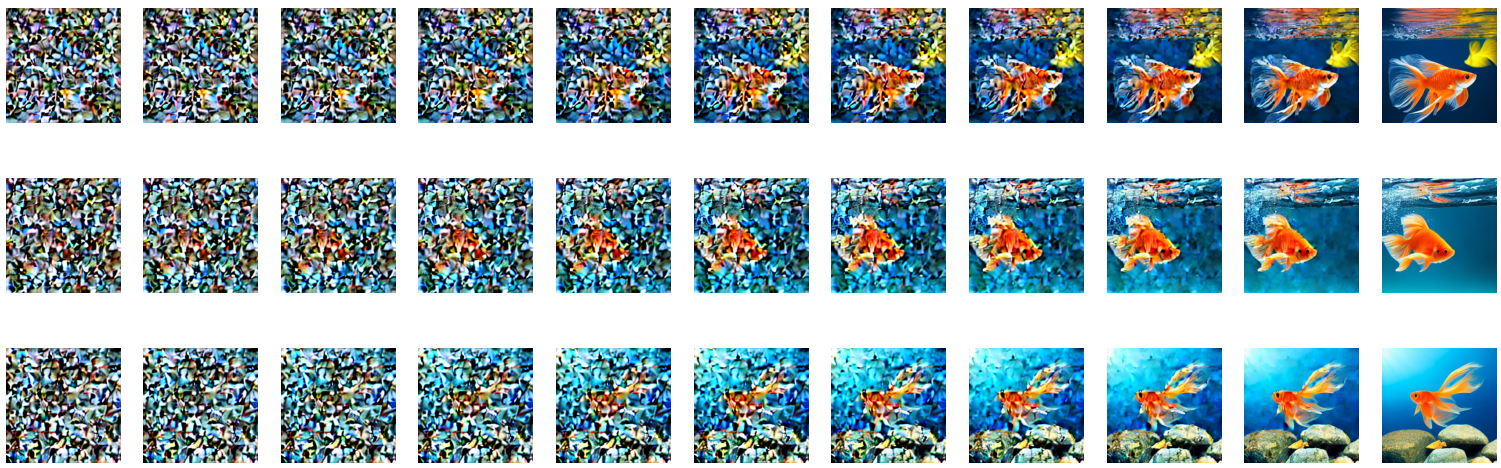
\includegraphics[width=150mm]{figures/sd_example_gf.png}
\caption{Example of a Stable Diffusion (MiniSD) generation. Prompt: ``A beautiful goldfish swimming through the ocean''. 50 steps, each 5th step drawn, three random noises used as starting points for the rows.}
\label{sd_generation_example}
\end{figure}

\paragraph{Introduction} On a high level of understanding, a pretrained SD model, just like any other DM, generates trajectories from the noisy space to the meaningful for us humans space by gradually removing noise from this random starting point. 
Figure~\ref{sd_generation_example} demonstrates three examples for such trajectories for the SD model that was used in this work.
The prompt is fixed for all these examples: ``A beautiful goldfish swimming through the ocean''.
The first column depicts three random noises that were used as starting points for the corresponding three trajectories that show the denoising process.
In this process, as we look at the pictures in each row from left to right, we observe the model gradually remove the noise to arrive at different finishing points. 
All three final generations in the last column, however, satisfy our conditioning requirement, which is the given prompt.

So, during the training process of a DM, noise is added to input images, and the main part of the model, normally its U-Net component, is training to predict the noise that was added at each step.
That way, during sampling, we are able to use this pretrained U-Net to go in the opposite direction of removing noise. 

Another important part of the process is conditioning, which in case of a SD model is usually added in the form of a text prompt, or more rarely a semantic map.
The conditioning is inserted into the U-Net with the use of attention, and the text itself is encoded with a CLIP model. 

Finally, a SD model is a latent diffusion model. 
Since we often want to work with large images that might take too much GPU memory, this class of models works on optimization in a latent space instead of the original pixel space of actual images. 
In order to work in this space, however, we have to be able to go into the space and leave it at will.
Typically, a Variational AutoEncoder (VAE) model is used for this purpose: its encoder allows the transition into the latent space, while its decoder returns latents to the corresponding images in the real pixel space.



\begin{figure}[ht!]
\centering
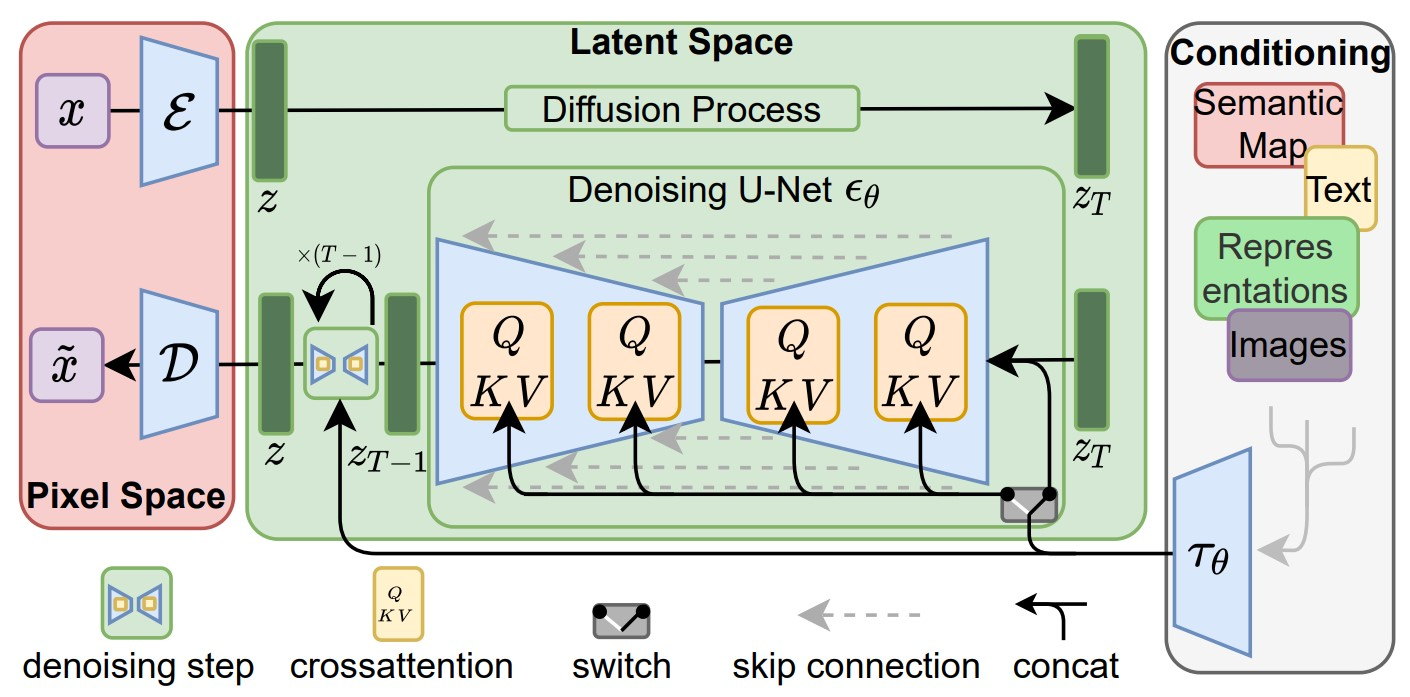
\includegraphics[width=120mm]{figures/sd.jpg}
\caption{Stable Diffusion Training Pipeline.}
\label{sd}
\end{figure}

\paragraph{Formalization} Now, let us turn to a little more low-level explanation with formulas and illustrations.

Figure~\ref{sd} depicts the pipeline in the scheme from the original paper~\cite{stable_dif}.
The leftmost red part indicates the pixel space with real images, and the green part---the training process that is happening in the latent space.
The transitioning between the spaces is possible with the use of a VAE with encoder $\mathcal{E}$ and decoder $\mathcal{D}$.
That is, a real image $x$ can be translated into a latent $z$ in the latent space by applying the encoder $\mathcal{E}$ of this VAE, while the reverse process is carried with the decoder $\mathcal{D}$: 
$$z = \mathcal{E}(x), \Tilde{x} = \mathcal{D}(z)$$

$\Tilde{x}$ is a reconstructed original image $x$. 
During training of a SD, the weights of its VAE model are fixed.

The forward diffusion process gradually adds noise to our original latent $z$ in $T$ steps, and the model trains to predict the previous latent $z_{t-1}$ for all $z_t$.
So, our SD is actually learning the original data distribution by learning how to reverse a fixed Markov Chain of length $T$.
A denoising U-Net model $\epsilon_\theta$ is used to predict the noise that can be used to obtain $z_{t-1}$.
The text prompt is included in the U-Net with help of cross-attention as shown on the picture: or conditioning $y$ is turned into its representation $\tau(y)$.
% TODO should I include the loss function for SD?

After training is completed, we obtain a U-Net model that can denoise our latents.
During sampling, we take a prompt and an initial latent, be it random or somehow conditioned, and then run the trained U-Net for several iterations to denoise it, apply our decoder $\mathcal{D}$ and obtain our final image $\Tilde{x}$.
Theoretically speaking, each iteration in the denoising sampling cycle improves our final result; in practice, however, for a simple generation without specific guidances, a relatively small number of iterations ($\lesssim 1e2$) is enough to obtain a meaningful realistic result.
On the contrary, since generation is performed with a fixed scheduler, it is impossible to run the cycle for an infinite number of iterations without altering the sampling process of the given pretrained model.

\paragraph{Guidance}\label{sec:guidance}
Apart from conditioning, there exist other methods that push the generation towards a particular desired direction.
Let us formally describe guidance, a method that can be used to ensure that our generated image is not random in the space of all generations that satisfy the prompt, but rather is somehow altered.
Let us take a look at the update formula for the latents in the diffusion sampling cycle in the simplest form starting from $z_T \sim \mathcal{N}(0, 1)$:
$$\hat\epsilon_t = \epsilon_\theta(z_t;t,y)$$

where $z_t$ is the latent at step $t$ and $y$ is our condition, typically a prompt.
As we have previously stated, in this formula, we are predicting an estimate of the noise that was added to $z_{t-1}$ in order to create $z_t$:
$$z_{t-1} = \text{scheduler}(z_t, \hat\epsilon_t, t)$$

where scheduler depends on our sampling method; our SD uses pseudo numerical methods for diffusion models.

% TODO talk about classifier guidance? 

It was, however, proven that for improving the quality of the image and for a better conditioning it it better to use classifier-free guidance~\cite{ho2022classifierfree}:
$$\hat\epsilon_t = (1+s)\epsilon_\theta(z_t;t,y) - s\epsilon_\theta(z_t;t,\emptyset)$$

where $s$ is a hyperparameter that determines the strength of classifier-free guidance and is typically set to 7.5.
Without this guidance, the conditioning is rather poor and the result might not correspond to our prompt well.
Let us also recall that since DMs in general are score-based, $\epsilon_\theta(z_t)$ estimates the score function for the intermediate noisy distributions between $z_t$ and $z_{t-1}$:
$$\epsilon_\theta(z_t) \approx -\sigma_t\nabla_{z_t} \log p(z_t)$$

Now we can take a look at sampling even in a more general light and learn how to add the an arbitrary guidance to the formula:
$$\hat\epsilon_t = (1+s)\epsilon_\theta(z_t;t,y) - s\epsilon_\theta(z_t;t,\emptyset) + v\sigma_t\nabla_{z_t}g(z_t; t, y)$$

here, $g$ can be any energy function that guides our generation in a meaningful way, $v$ is self-guidance weight and $\sigma_t$ converts the score function to a prediction of $\epsilon_t$.

\paragraph{MiniSD} It is also important to note that due to our GPU resources limitations, we were unable to use the standard SD and used MiniSD from Hugging face instead; compared to its standard version, the MiniSD can generate images at resolution 256 without a noticeable loss in quality.

\subsubsection{YOLO}

\begin{figure}[ht!]
\centering
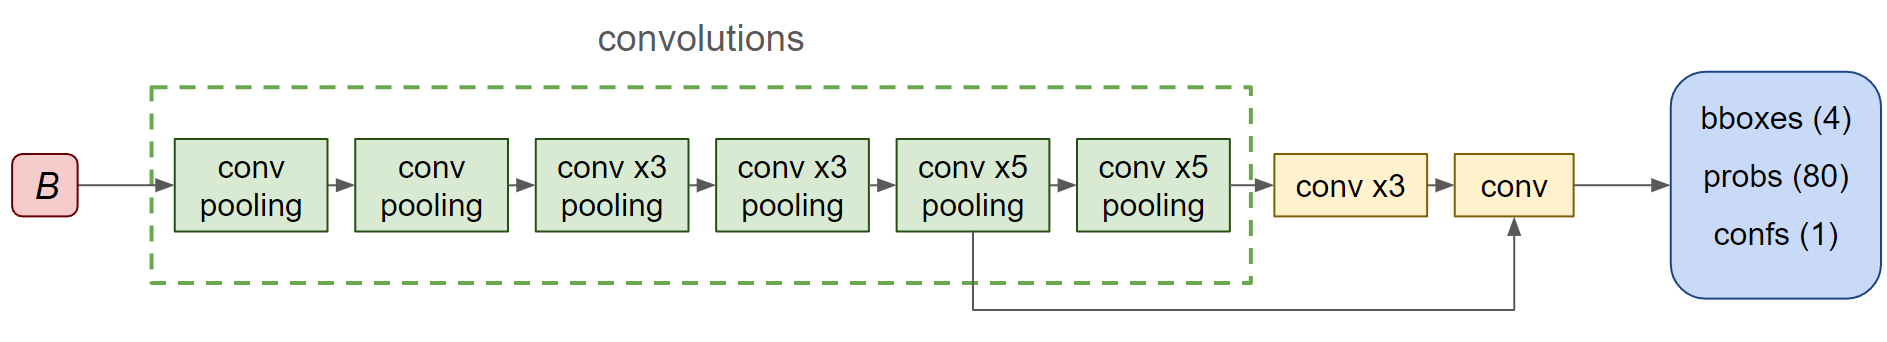
\includegraphics[width=150mm]{figures/yolov2.png}
\caption{Darknet-19, detection pipeline.}
\label{darknet19_detection}
\end{figure}

Another important model that we use in our pipeline is YOLO.
Figure~\ref{darknet19_detection} shows the architecture of the Darknet-19 that was introduced in the paper as a model that can be used for classification and detection. 
More specifically, in general, only the green part of the scheme is Darknet; the depicted architecture is a Darknet modification that is used for detection. 
When the yellow follow-up convolutions are replaced with another single convolution, the model becomes its classification Darknet-19 modification; they are trained jointly in the original paper.

The pipeline itself is very simple. 
In the simplest case, for a detection Darknet, a batch of square input images $B$ of size $3\times 416\times 416$ goes through the convolutions and poolings until the final predictions are obtained.
As it has been mentioned previously, the output data of YOLO consists of three parts: bboxes that show the positions of the predictions, probabilities for all classes, and confidences in predictions. 
Since each bbox is defined through its position and size, all of them are predicted in four values.
YOLOv2 specifically was trained for the COCO dataset~\cite{cocodataset}, the Darknet model returns probabilities for 80 classes. 
The confidence, or the objectiveness score, predicts the IoU between the proposed bbox and the ground truth label. 
The architecture also contains a shortcut as shown on Figure~\ref{darknet19_detection} to make the model take fine-grain features into consideration.
Each convolutional layer in the scheme is followed by batch normalization as regularization to speed up convergence and stabilize the training process. 

Another trick that is used in YOLO is anchors. 
After the batch of images $B$ goes through all the convolutions, we obtain feature maps for the images of size $13\times 13$, which can be understood as positions on the images. 
For each of these positions, our model learns to predict offsets for $5$ anchors that denote most cluster centers for object sizes of training dataset. 
That is, the authors chose the number of clusters for all object sizes in the training data as $5$ (the number chosen empirically), and then, instead of actually predicting the size of the object in the grid, we predict offsets to these anchors; centers of objects, that is, their positions, are also predicted as offsets from the central positions in the grid.
So, to sum up everything that has been mentioned, the final output has size $\text{batch\_size}\times 13 \times 13\times 5\times (4 + 1 + 80)$.

% TODO details on YOLO?

\subsection{General Pipeline}

In this section, we will introduce the general pipeline we used for our adversarial generations.

\begin{figure}[ht!]
\centering
\subcaptionbox{Original SD\label{sd_my-a}}{
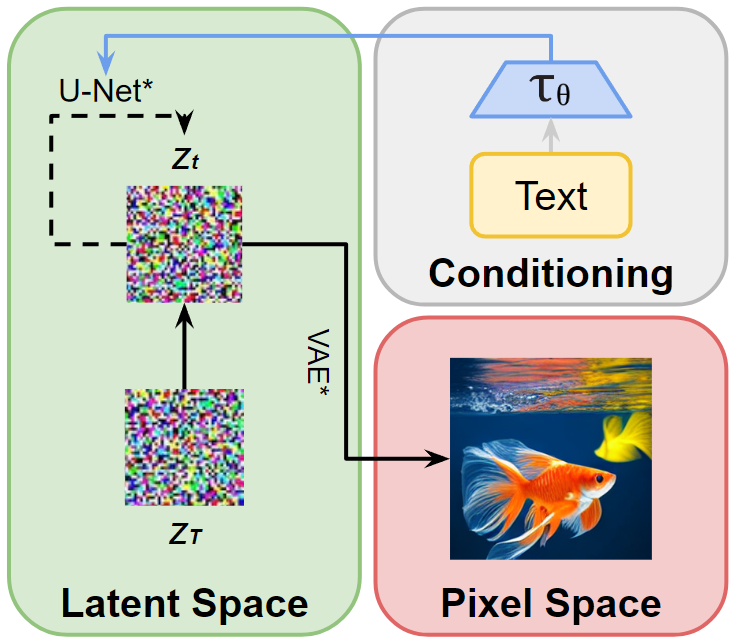
\includegraphics[width=0.45\linewidth, trim={0 0 0 0}]{figures/sd_my.png}
}
\subcaptionbox{Modification: adversarial guidance\label{sd_my-b}}{
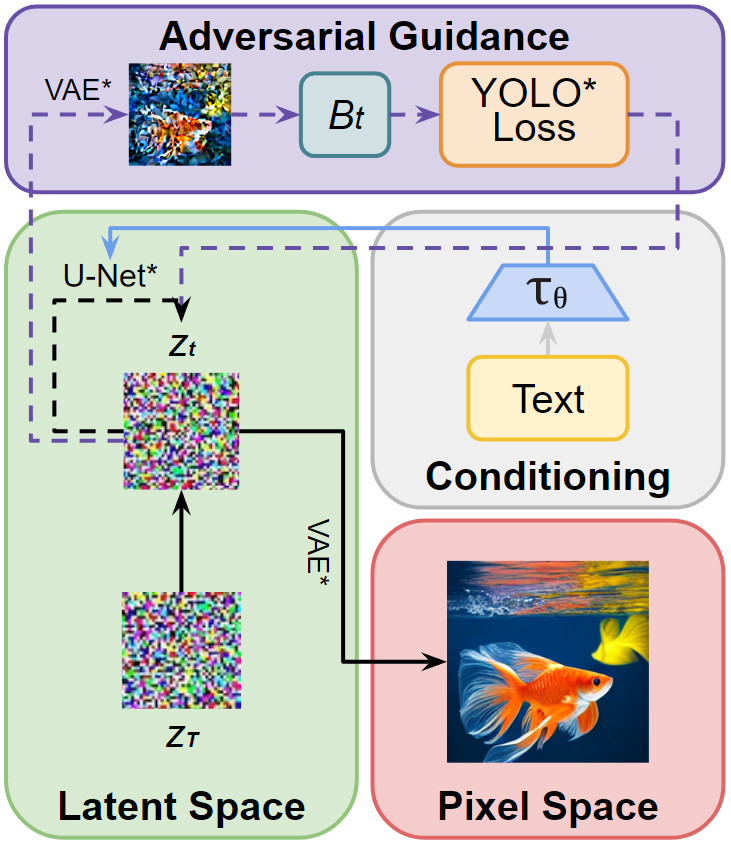
\includegraphics[width=0.45\linewidth, trim={0 0 0 0}, clip]{figures/sd_my_adv_common.png}
}
\caption{Stable Diffusion: original and modified pipelines.}
\label{sd_my}
\end{figure}

Figure~\ref{sd_my-a} depicts the original SD pipeline that was already introduced in Figure~\ref{sd}, albeit in a simplified form with the insides of U-Net hidden.
The sampling cycle that goes on for $T$ iterations is indicated by the gray dashed line: the U-Net model, taking into account the conditioning, predicts noise that should be removed from the latents at each step. 
After the cycle is completed, we leave the latent space for the pixel space with the help of VAE's decoder $\mathcal{D}$.

Figure~\ref{sd_my-b} introduces changes to this process.
Overall, the sampling pipeline stays the same, but we add a correction to our update direction in the form of adversarial detection guidance. 
That is, during the sampling process, we want to guide our latent not only towards generating a specific image according to our prompt conditioning, but also make it adversarial. 
Let us recall the guidance formula in general: 
$$\hat\epsilon_t = (1+s)\epsilon_\theta(z_t;t,y) - s\epsilon_\theta(z_t;t,\emptyset) + v\sigma_t\nabla_{z_t}g(z_t; t, y)$$

In order to define adversarial guidance, we have to understand what the energy function $g$ looks like in this case.
In essence, the energy function $g$ is some kind of adversarial detection loss; more formally, 
$$g(z_t; t, y) = s^{adv}_t \cdot \text{adv\_loss}(z_t, \mathcal{D}, \text{YOLO}, B_t)$$

where:

\begin{itemize}
    \item $s^{adv}_t$ is the adversarial guidance coefficient at step $t$. 
    It makes sense to change the intensity of adversarial guidance through the sampling process, so the entire set of adversarial guidance coefficient, $S^{adv} = \{s^{adv}_t\}^T_1$, is an important hyperparameter that will be later referred to as adversarial guidance scheduler;
    \item $z_t$ is intermediate latent that can be decoded into the corresponding intermediate noisy image $\Tilde{x_t}$ in the pixel space with VAE decoder: $\Tilde{x_t} = \mathcal{D}(z_t)$; 
    \item YOLO is our object detection model that is the key to obtaining the adversarial guidance; 
    \item $B_t = \{X_t, L_t\}$ is a batch of object detection images consisting of images $X_t$ and their labels $L_t$; 
    \item adv\_loss is our current method to extract the component of the real YOLO loss that is relevant to the task. 
    In our case, since we are working on evasion attacks, it will be the objectiveness score; in the general case, it can be any other meaningful part of the YOLO output, such as, for instance, the probabilities of predicted classes or bboxes.
\end{itemize}

Since $B_t$ mostly depends on the chosen pipeline type, further explanations of the formula will be introduced in the appropriate sections below.

Overall, the main idea is to alter the update direction of the conditioned update to arrive at an adversarial sample, much like classifier guidance from~\cite{dhariwal2021diffusion}.

\subsection{Adversarial Guidance Pipelines}

We have tried two techniques for calculating YOLO loss based on different approaches to obtaining data $B_t$ and applying $x_t$ to this data.
The pipelines are called 2D and 3D.
In the first pipeline, we use images from an existing labeled dataset with people, Inria Person~\cite{inria}.
$x_t$ are attached to the people from batch $B_t$ as patches.
With 3D pipeline, the background dataset~\cite{zh_3d} does not contain people; instead, human figures are dressed in clothes with tiled generations and rendered with certain augmentations.

\begin{figure}[htp]
\subfloat[2D]{
  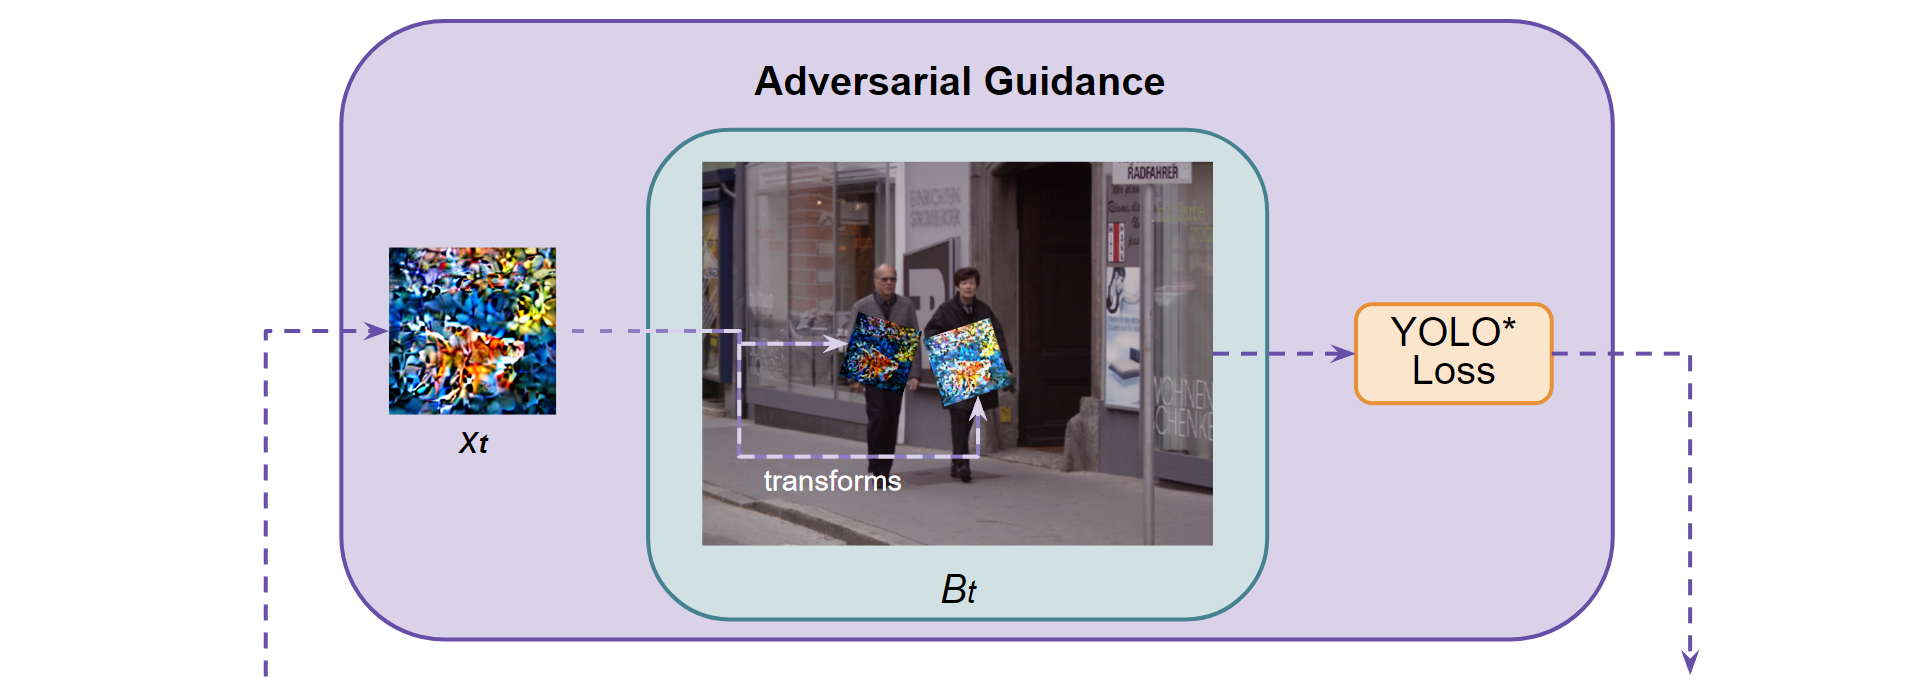
\includegraphics[clip, width=\columnwidth]{figures/sd_adv_2d.png}\label{ad_guid_a}
}\hfill
\subfloat[3D]{
  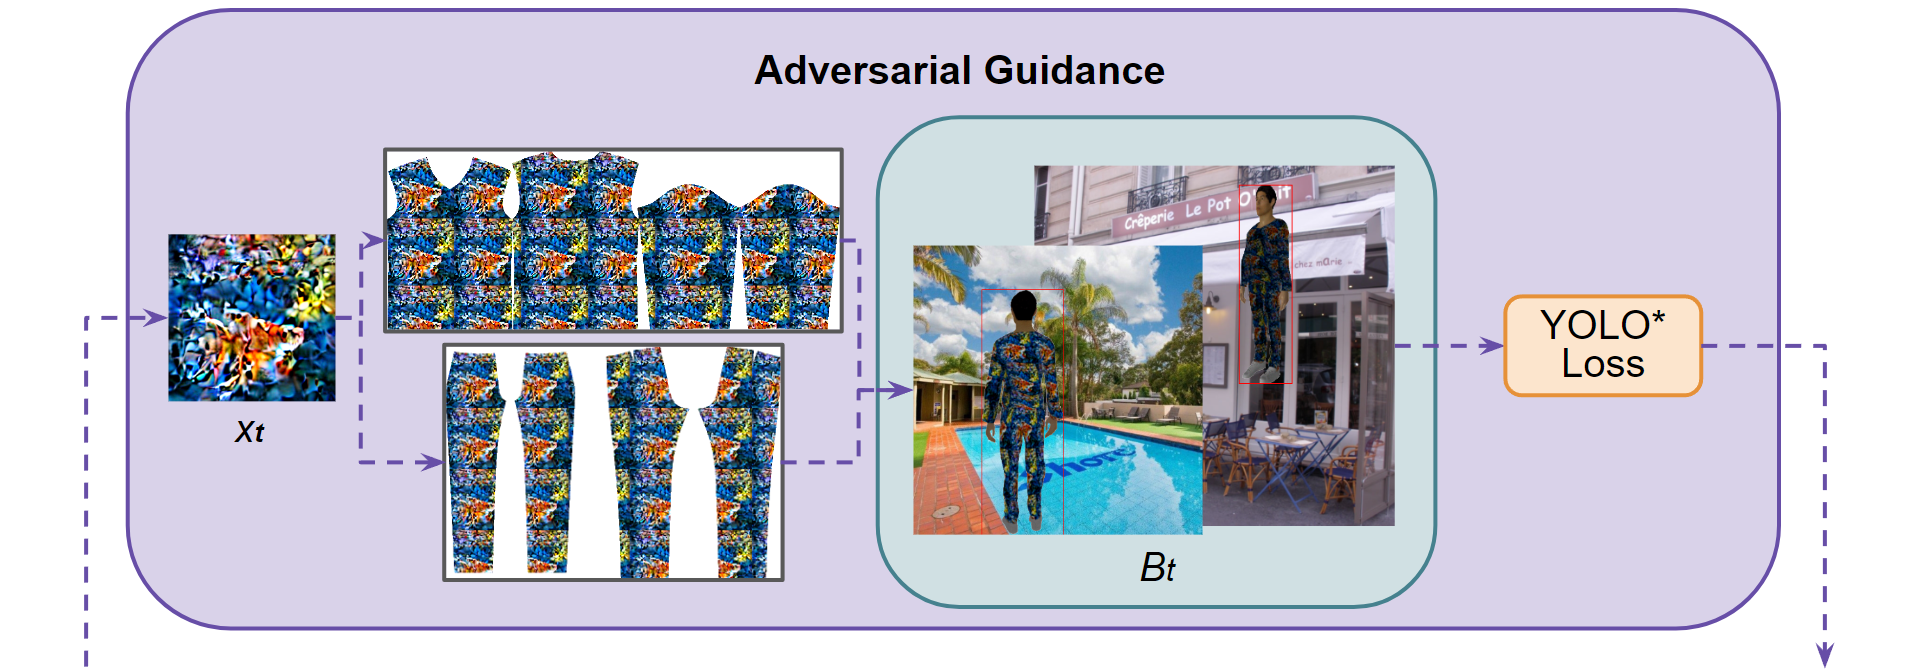
\includegraphics[clip, width=\columnwidth]{figures/sd_adv_3d.png}\label{ad_guid_b}
}
\caption{Adversarial Guidance Pipelines}
\end{figure}

The pipelines are shown on Figures~\ref{ad_guid_a} and~\ref{ad_guid_b}.


\paragraph{2D} In the case of 2D pipeline, intermediate partially denoised images $x_t$ are attached to all people from every image $X_{tm}$ in batch $B_t = \{(X_{tm}, L_{tm})\}_1^M$ consisting of $M$ images.
We are trying to lower the highest confidence of relevant bboxes, so the energy function in this case is:
$$g(z_t; t, y) = s^{adv}_t \sum_{m=1}^M \max \text{\LARGE [} \text{yolo\_loss}\text{\large (}\Tilde{X}_{tm}, L_{tm}\text{\large )}_{\text{obj}} \text{\LARGE ]}$$

where $\Tilde{X}_{tm}$ is $X_{tm}$ with attached augmentations of $x_t$, yolo\_loss is the regular loss for the YOLO, and $_{\text{obj}}$ signifies that we only look at the objectiveness (confidence) scores of the predictions, since we are performing an evasion attack and want to not be detected. 

In this case, augmentations consist of the standard simple transformations like adjustments of brightness, angle, contrast, and adding random noise, and also applying Thin plate splines (TPS, see Section~\ref{sec:tps} below).
All of the applied transformations are differentiable. 

\paragraph{3D} 
In the case of 3D adversarial guidance pipeline, we first tile our generated texture $x_t$ to cover a 3D model's clothes $C_t$.
Afterwards, using a 3D rendering module of Python, we render a 3D model that we have prepared in advance with help of~\cite{zh_3d}.
The models are rendered on random backgrounds from the dataset.
We also sample light and camera angles to ensure the effectiveness of our attack in the real world. 
This, as well as the 3D TPS, TopoProj (see Section~\ref{sec:tps}),  and shifting of the initial position of $x_t$ on $C_t$, are our augmentations.

The energy function is essentially the same as in the 2D case, albeit it is important to note that in this case, labels $L_{tm}$ are not provided in the dataset, but rather calculated according to the current sampling and rendering strategy that changes over time, and images $X_{tm}$ contain rendered figures as shown on Figure~\ref{ad_guid_b}.

\subsection{TPS and TopoProj}\label{sec:tps}

One of the most important augmentations we use in this task is TPS. 

 TODO 

Another important technique that was introduced in~\cite{zh_3d} is TopoProj.

 TODO 

% \subsection{Obtaining Latents}

% The simplest way to obtain the latent corresponding to an input image is to take the encoder part of the pretrained diffusion model, $\mathcal{E}$ from Figure~\ref{sd}.
% Otherwise, it is also possible to use the paper called ``Null-text Inversion for Editing Real Images using Guided Diffusion Models'' for obtaining the latent.
% In this paper, the authors introduce a method to improve the basic DDIM inversion so that it works better with classier-free guidance that is also used in our main pipeline.


\section{Appearance Restoration}

As we have stated previously, we want our adversarial evasion clothes to be controllable: that is, we are able to obtain not just a random adversarial pattern, but rather be able to make it closer to something we want to see specifically.
Let us say we have a simple non-adversarial sampling trajectory of our SD $\hat{z}_T\ldots\hat{z}_0$ that leads us to our desired image $\hat{x} = \mathcal{D}(\hat{z}_0)$.
Now we are trying to generate $x$, an adversarial texture for clothes that at the same time is close to our original $\hat{x}$.
Firstly, we make a step according to our U-Net prediction; secondly, this direction is modified with adversarial guidance. 
The trajectory, however, can change significantly compared to the original one, so $x$ can be very different from $\hat{x}$ if the adversarial scheduler $S^{adv}$ consisted of large coefficients.

So, we have to propose a method to preserve the original appearance, even maybe at the cost of adversarial effectiveness. 
In order to do that, we insert additional appearance restoration guidances that push our generation in the direction of the original sampling trajectory.
We have tried guidances dictated by two different losses that we will introduce in this section.

\subsection{Appearance Constraint Loss}

Since the attention maps of U-Net contain information about the position and the form of objects and the activations from appropriate layers store the appearance of the objects, it is possible to manipulate several properties of the objects using the representations stored in the U-Net layers.
% TODO 

Following~\cite{aibek}, let us define the appearance of objects in terms of the information stored in U-Net.
Let us denote an intermediate attention map from layer $n$ on timestamp $t$ as $\mathcal{A}_{t,n} \in \mathbb{R}^{P \times H_n\times W_n}$, where $P$ is the length of the prompt (one word is one channel starting with position 1; empty tokens are added at the end until we reached the intended length $P$).
Similarly, activation (features) will be denoted as $\mathcal{F}_{t,n}\in \mathbb{R}^{F_n\times H_n\times W_n}$.

According to~\cite{att_replace_silver_robots}, attention maps store information about the shape and the position of the objects from their corresponding channels.
That is, by looking at the attention maps $\mathcal{A}_{t,:}$ at timestamp $t$, we can see the shape of all objects; if we want to see the shape of $p$-th object from layer $n$, we should look at $\mathcal{A}_{t,n,p}$.
The bigger the value in the corresponding channel, the more related the pixels are to this word.
Omitting timestamps and layering indexing, the following formula can be used to calculate the shape of object $p$:
$$\text{shape}(p) = \mathcal{A}_p$$

In practice, attention maps $\mathcal{A}$ are thresholded to account for background noise. 
It is possible to change the shape of object by guiding these maps towards those of another generation or provided by the user, but in our case, we are interested in the entire appearance of objects that can be expressed as:
$$\text{appearance}(p) = \dfrac{\sum_{h,w}\text{shape}(p)\odot \mathcal{F}}{\sum_{h,w}\text{shape}(p)}$$

This formula makes sense because $\text{shape}(p)$ creates a mask that denotes the form of object $p$ and activation maps represent local appearance.

To use appearance constraint as guidance, we need to define the energy function $g$.
As we have mentioned in the introduction part of this section, we already have our original generation $\hat{x}$ and latent trajectory that leads to it. 
That is, we can run the SD to obtain this trajectory $\hat{z}_T\ldots\hat{z}_0$.
While running this process, we can store all the intermediate U-Net attention maps and activations to be able to reconstruct the original $\widehat{\text{appearance}_t(p)}$ for object $p$ on timestamp $t$ of this original run.
With this, we can use attention constraint guidance as the gradient obtained from the l1-loss between the original appearance and the current appearance of object $p$:
$$g(t, p) = s^{ap}\cdot \text{l1-loss}(\text{appearance}_t(p), \widehat{\text{appearance}_t(p)})$$

where $s^{ap}$ is the corresponding guidance coefficient.

In our case, we want the entire generation to be close to the original, so we add the guidance to all words in the prompt as $\sum_{p\in P} g(t,p)$.

\subsection{Attention Constraint Loss}

Even though the method helps to fix the appearance of the generation, fixing all words is a prompt has little physical meaning.
For example, for a prompt ``a beautiful goldfish swimming through the ocean'', it is easy to imagine what objects like ``goldfish'' and ``ocean'' do look like, but it fixing parts of prompt like ``a''/``through'' or ``swimming'' is unjustified.
This is why we suggest to only fix self attention maps that restrict the affinities between the features. 
Self-attention maps control the layout of the image in the lower layers and capture details on higher, so guiding them will guide the entire image to the original $\hat{x}$.

Similarly to appearance constrain loss, we have to run the original trajectory $\hat{z}_T\ldots\hat{z}_0$ and store all self-attention maps $\hat{\mathcal{A}}^{self}_t$ on all timestamps $t$.

The guidance can be defined as l1-loss for the original and newly generated self-attention maps:
$$g(t) = s^{at}\cdot \text{l1-loss}(\mathcal{A}^{self}_t, \hat{\mathcal{A}}^{self}_t)$$

TODO for this and previous subsections: illustrations (?)

\section{Final Algorithm for 3D Pipeline}

\begin{figure}[ht!]
\centering
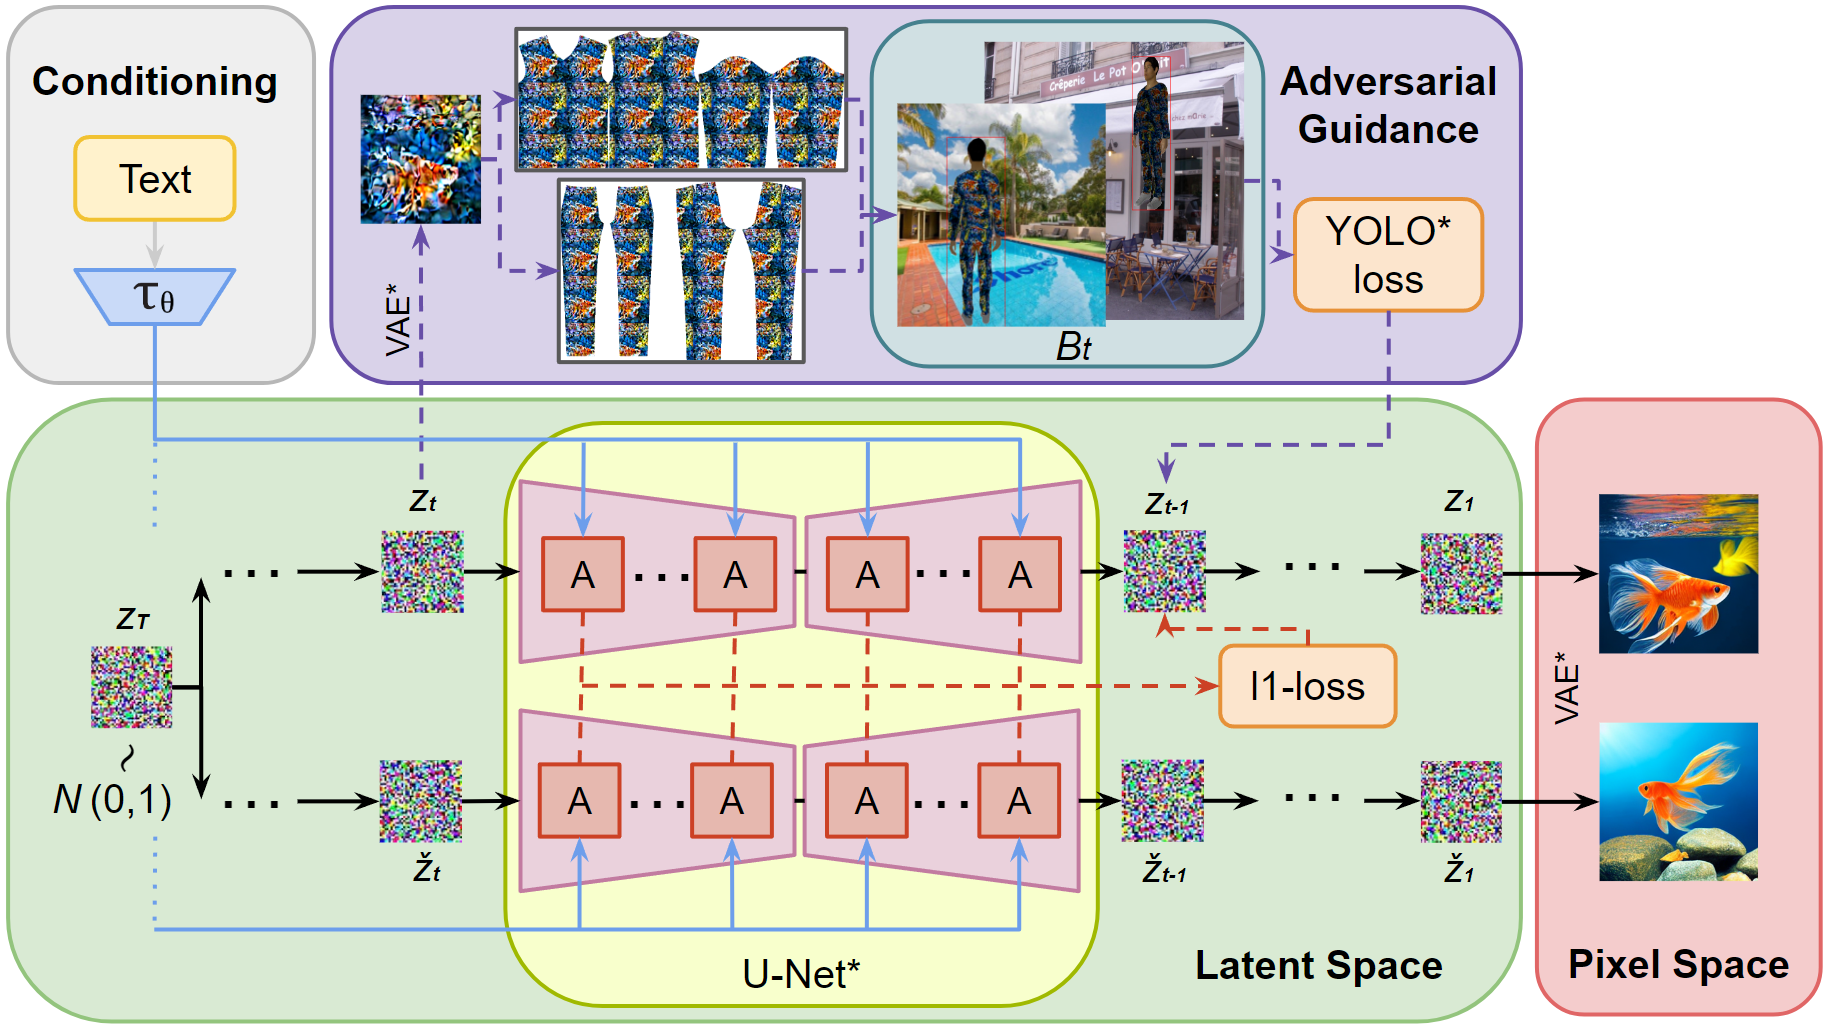
\includegraphics[width=150mm]{figures/sd_adv_fix_3d.png}
\caption{Final pipeline with both adversarial and fixation guidances.}
\label{sd_3d_adv_fix}
\end{figure}

In our case, for the $g$ energy function, we chose YOLO loss.
Again, the physical explanation of this guidance is that we are trying to maximize YOLO loss for the predicted people, so that ultimately our patch helps in avoiding detection by this YOLO:
$$\nabla_{z_t}g(z_t; t, y) = s^{adv}_t \sum_{m=1}^M \nabla_{z_t}\max \text{\LARGE [} \text{yolo\_loss}\text{\large (}\Tilde{X}_{tm}, L_{tm}\text{\large )}_{\text{obj}} \text{\LARGE ]}$$

So, compared to the standard SD sampling, we allow latent $z_t$ to accumulate gradients and add this gradient to our update $\hat\epsilon_\theta$.
In this section, we will provide the adversarial algorithm for our pipeline that is fully shown in Figure~\ref{sd_3d_adv_fix} on the example of the combination of two guidances: adversarial and attention constraint.


\renewcommand{\algorithmicrequire}{\textbf{Inputs:}\unskip}
\renewcommand{\algorithmicensure}{\textbf{Output:}\unskip}
\renewcommand{\algorithmiccomment}[1]{\textcolor{gray}{{\scriptsize$\triangleright$}\,#1}}


\begin{algorithm}
  \caption{Sample adversarial $x$ based on non-adversarial $\hat{x}$}
  \label{alg1}
  \small
  \begin{algorithmic}
    \REQUIRE Prompt $\mathcal{P}$, number of SD steps $T$, adversarial scheduler $S^{adv}$, attention constraint coefficient $s^{at}$, adversarial dataset $DS$

    \STATE $z_T \sim \mathcal{N}(0, 1)$\hspace{2.38cm}
    \COMMENT{initial noisy latent}
    
    \STATE $P_{emb} \gets \tau(\mathcal{P})$\hspace{2.5cm}
    \COMMENT{CLIP prompt encoding}

    \STATE {$\text{self\_att\_maps} \gets []$} 
    \FOR{$t \leftarrow T$ to $1$}
        \STATE {$\text{self\_att\_maps.register(U-Net.self\_attention)}$}\quad
	\COMMENT {saving attention maps for non-adv sampling}
        \STATE $\epsilon \gets \text{U-Net}(z_t, P_{emb})$
        \STATE $z_{t - 1} \gets \text{update}(z_t, \epsilon)$
    \ENDFOR

    \FOR{$t \leftarrow T$ to $1$}
        \STATE $\epsilon \gets \text{U-Net}(z_t, P_{emb})$
        \STATE $x_t \gets \mathcal{D}(z_t)$\hspace{2.32cm}
	\COMMENT{decoding latents into intermediate images}

	\STATE $X, L = DS\text{.next\hspace{0.05cm}}()$
        \STATE $\Tilde{X} \gets X.\text{attach}(x_t)$\hspace{1.3cm}
	\COMMENT{obtaining augmented image for YOLO}

        \STATE $\epsilon \gets \epsilon + S^{adv}_t\nabla_{z_t}\text{YOLO-loss}(\Tilde{X}, L)$\hspace{4.127cm}
	\COMMENT{adv guidance}

        \STATE $\epsilon \gets \epsilon + s^{at}\nabla_{z_t}\text{l1-loss(U-Net.self\_attention, self\_att\_maps[t])}$\quad
	\COMMENT {appearance guidance}

        \STATE $z_{t - 1} \gets \text{update}(z_t, \epsilon)$
    \ENDFOR

    \STATE $x \gets \mathcal{D}(z_0)$
    \ENSURE Adversarial $x$
  \end{algorithmic}
\end{algorithm}

The method is shown in algorithm~\ref{alg1} in pseudocode. 
Just as the usual SD pipeline, we start by generating the initial noisy latent $z_T$ (in case it was not provided by the user in the input data).
We also have to use our text encoder, typically CLIP, to create prompt embeddings $P_{emb}$.

After that, we run the first sampling that is non-adversarial.
We need to do this since we intend to save attention maps from all intermediate steps to be able to guide our adversarial trajectory in the direction of the original path.
So, during the first cycle, we save all needed information from U-Net, which, in case of attention constraint guidance, are self-attention maps only.
The cycle itself is standard for SD: we generate noise prediction $\epsilon$ with the U-Net model and then use it to update the current latent $z_t$. 
In the actual pipeline, we also use classifier-free guidance described in Section~\ref{sec:guidance} by running the U-Net model for two inputs simultaneously, but this part is omitted in the pseudocode for its irrelevance to this method as it is used for improving results in general rather than its adversarial effects.

After the initial self-attention maps are stored, we can start running the adversarial sampling.
Now, on each iteration of standard SD sampling, we perform the following additional operations after obtaining noise prediction $\epsilon$ on step $t$:

\begin{enumerate}
    \item Use our frozen VAE model (decoder $\mathcal{D}$ from Figure~\ref{sd}) to obtain $\hat x_t$;
    \item Transform this $\hat x_t$ into clothes $\hat c_t$ for our 3D model;
    \item Render human figures dressed into the clothes $\hat c_t$ into scenes from the background dataset while performing augmentations to ensure effectiveness in physical attacks to create images $\Tilde{X}$ for YOLO;
    \item Calculate the YOLO detection loss for the scenes with our augmented $\Tilde{X}$ and their labels $L$;
    \item Perform adversarial guidance: add gradient $\nabla_{z_t}$ from this loss to the noise prediction $\epsilon$ with coefficient $S^{adv}_t$;
    \item Calculate the l1-loss between the current self-attention maps of U-Net and those we have saved from the original run;
    \item Perform attention constraint guidance: add gradient of the loss in the previous step to the noise prediction $\epsilon$ with coefficient $s^{at}$.
\end{enumerate}

Each iteration of the cycle is finished with updating latent $z_t$ with obtained guided noise $\epsilon$.

After the sampling cycle is completed, we can obtain our final adversarial $x$ as the decoded final latent: $x = \mathcal{D}(z_0)$.

\section{Tiling}

So far, we have not discussed why our method is natural considering the fact that we simply tile generated pictures are not necessarily tileable.
However, the section with experiments will show examples of generated patches that can be tiles almost seamlessly.
In this section, we describe our original method to achieve this effect without any additional guidance.

\paragraph{Prompt Modification}

\begin{figure}[htp]
\subfloat[Two levels of prompt extensions: the second level (the last row) contains patterns that can be tiled.]{
  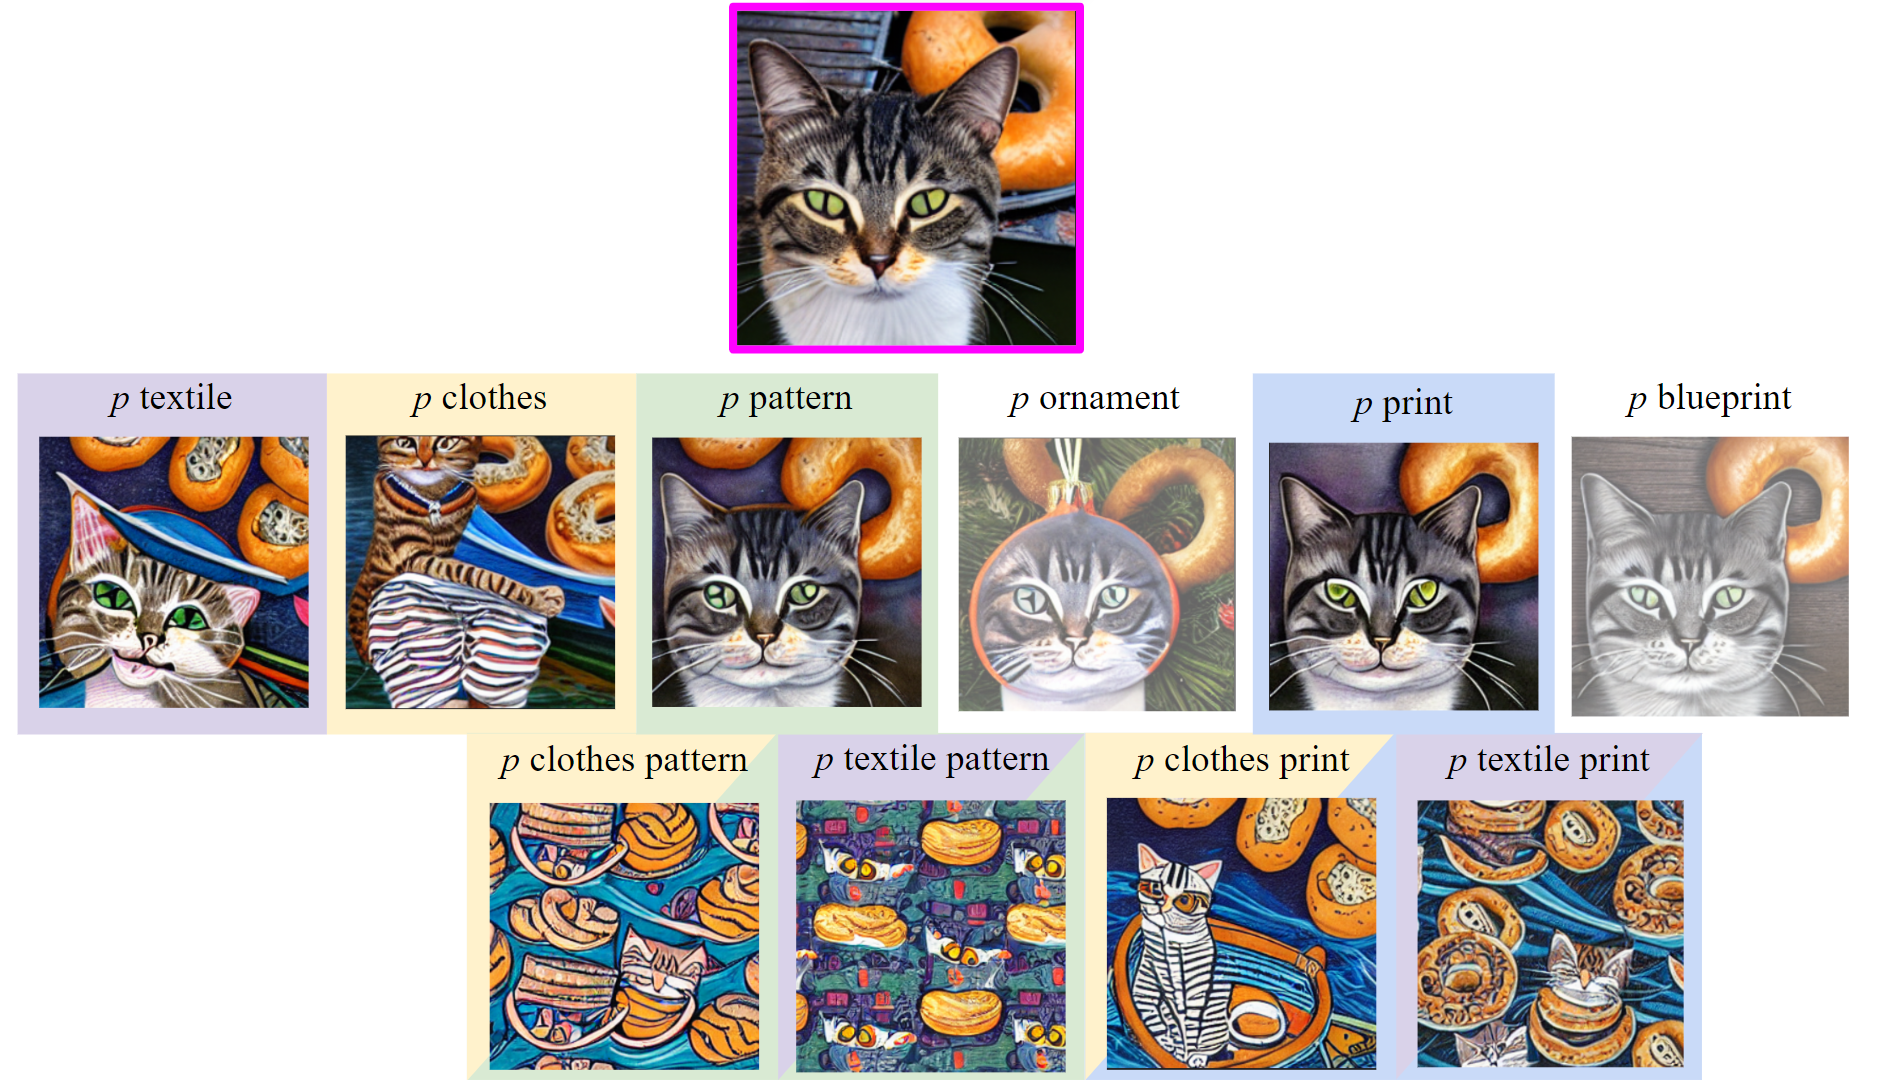
\includegraphics[clip, width=\columnwidth]{figures/tiling1.png}\label{tiling_a}
}\hfill
\subfloat[Stacking specific lines increases the effect.]{
  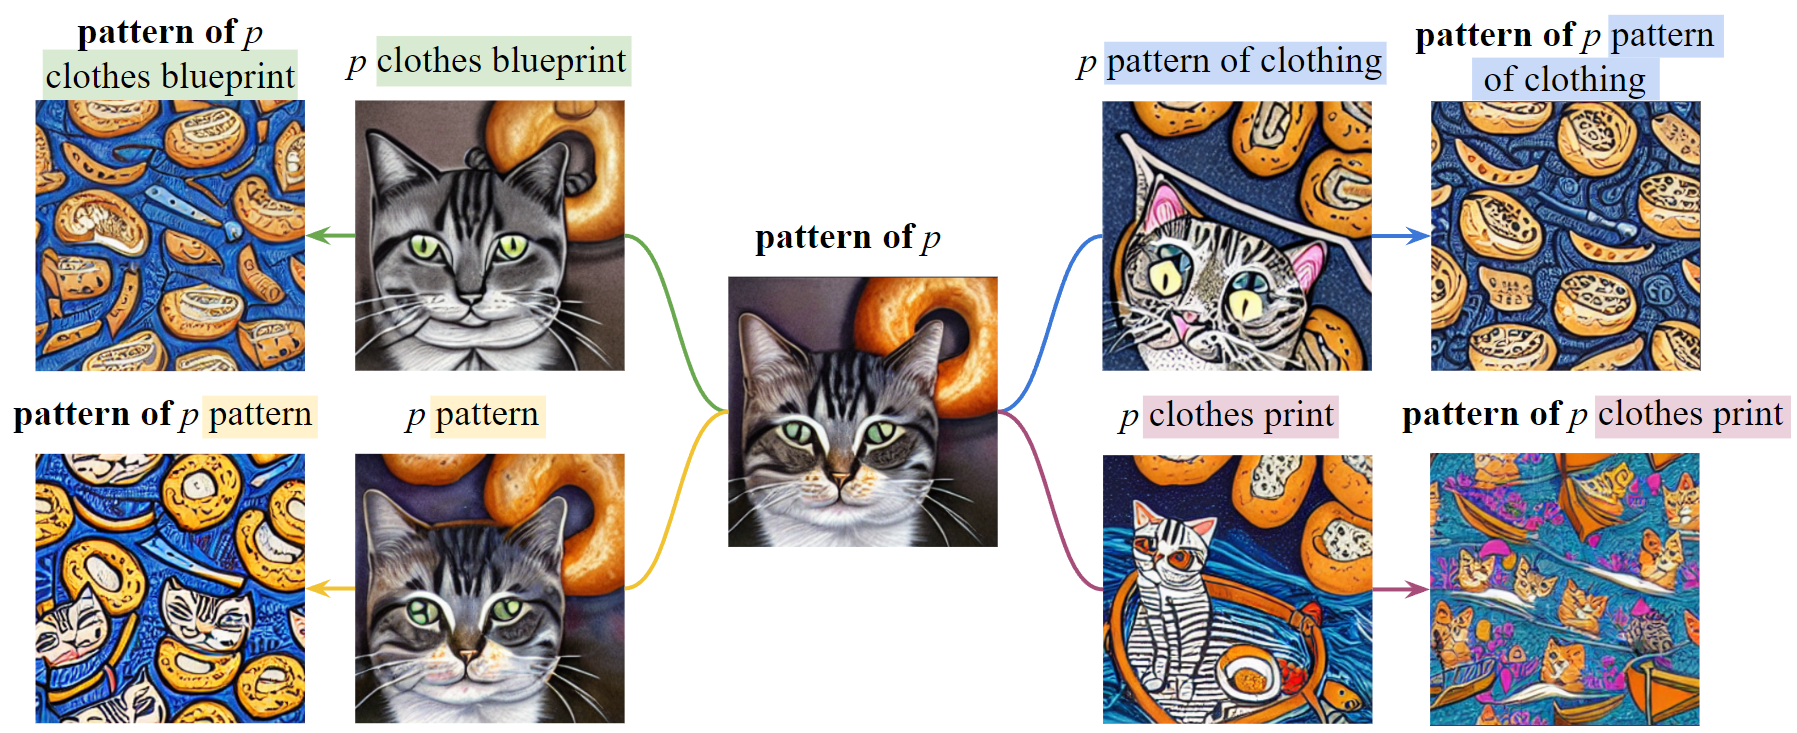
\includegraphics[clip, width=\columnwidth]{figures/tiling2.png}\label{tiling_b}
}
\caption{Prompt modifications for prompt $p$ ``A cat on a boat with a bagel'' (the highest image in a dark pink box).}
\end{figure}

The SD model is trained on a large dataset LAION~\cite{laion} that consists of roughly 5 billion images, so the model manages to learn many nuances of the text-image relationship, which can be used by modifying the input prompt.
It turns out that it is possible to modify the prompts to make the SD produce textures that can be tiled almost seamlessly.

Figure~\ref{tiling_a} shows several such examples.
In the upper row, we have the original generation for a random prompt --- ``A cat on a boat with a bagel''.
In the second row, we extend this prompt by adding one word that is related to our task, but do not obtain tileable textures just yet. 
In the last row, we show some of the combinations of the prompt extensions above. 
Three of them, ``\textit{p} clothes pattern'', ``\textit{p} textile pattern'', and ``\textit{p} textile print'' achieve the needed effect: if we put any of these generations side by side with itself, the final pattern will be smooth.
However, only a limited number of such combination works, and, for example, combining words ``\textit{p} textile'' and ``\textit{p} pattern'' with ``\textit{p} ornament'', and ``\textit{p} blueprint'' yield no needed results, and the generated patterns for these combinations in essence look like ``\textit{p} clothes print'' in the last row, which can not be tiled.

Interestingly, stacking these lines, we can enhance the effect, turning generations even for the non-effective first level extensions tileable.
Examples of this are shown on Figure~\ref{tiling_b}.
This set of examples for the same prompt demonstrates the effectiveness of the prompt command ``pattern of \textit{p}''.
By itself, as we can see from the image in the middle, the word does not make our random prompt generation continuous.
The same goes for four other prompt extensions that are connected to the image in the middle: ``\textit{p} clothes blueprint'' (green), ``\textit{p} pattern'' (yellow), ``\textit{p} pattern of clothing'' (blue), and ``\textit{p} clothes print'' (purple).
However, if we combine the original ``pattern of \textit{p}'' with any of the four aforementioned extensions, we will obtain the outer set of four images that can be put side by side to create continuous patterns.

\paragraph{Tiling vs Adversarial Effect}
% TODO theres no conflict

\begin{figure}[htp]
\centering
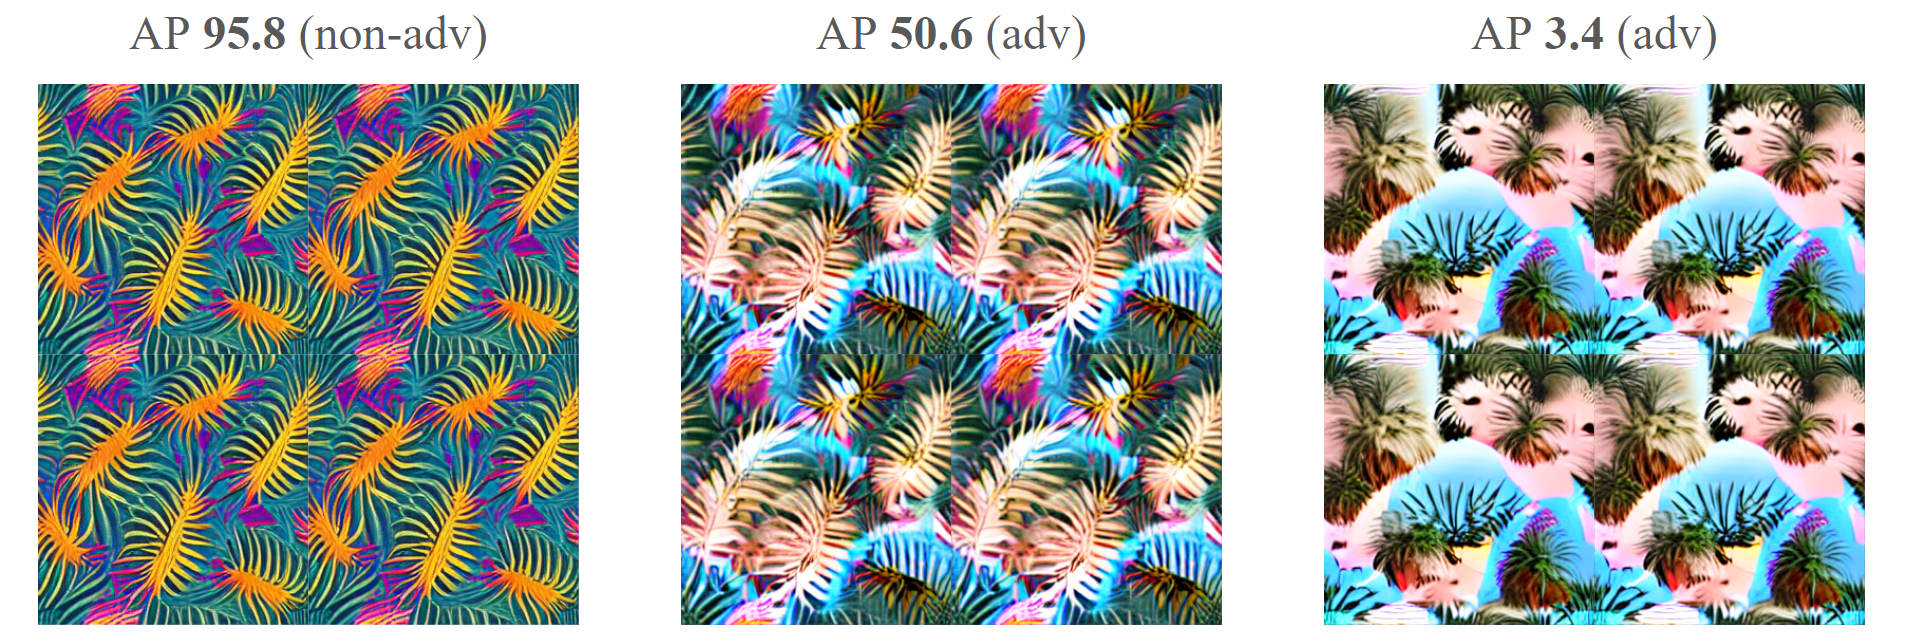
\includegraphics[width=150mm]{figures/adv_vs_tiling.png}
\caption{The generations are still tileable as we apply stronger adversarial guidances.}
\label{tiling_vs_adv}
\end{figure}

Importantly, this effect does not diminish as we add adversarial guidance to our generation.
To demonstrate this, we show three generations for the same prompt, ``palm clothes pattern'', in Figure~\ref{tiling_vs_adv}, which also shows what we mean by ``tileable'' images.
Here, in the left part, we have the original non-adversarial generation for the prompt repeated 4 times to demonstrate that the tiling has indeed almost negligible seams on the joints.

The next two parts of the figure show examples of adversarial and appearance-restorated generation for the same prompt. 
The middle one has little adversarial effect due to the weak adversarial scheduler and strong attention and appearance constraining guidance coefficients, so the average precision (AP) is rather high.
At the same time, the rightmost part shows an example of a highly adversarial image with little resemblance to the original generation. 

Yet all of these three generations can be tiled very well, and a stronger adversarial scheduler does not mitigate the tiling prompt extension, which, in this case, is ``clothes pattern''.

\paragraph{Problems}

\begin{figure}[htp]
\centering
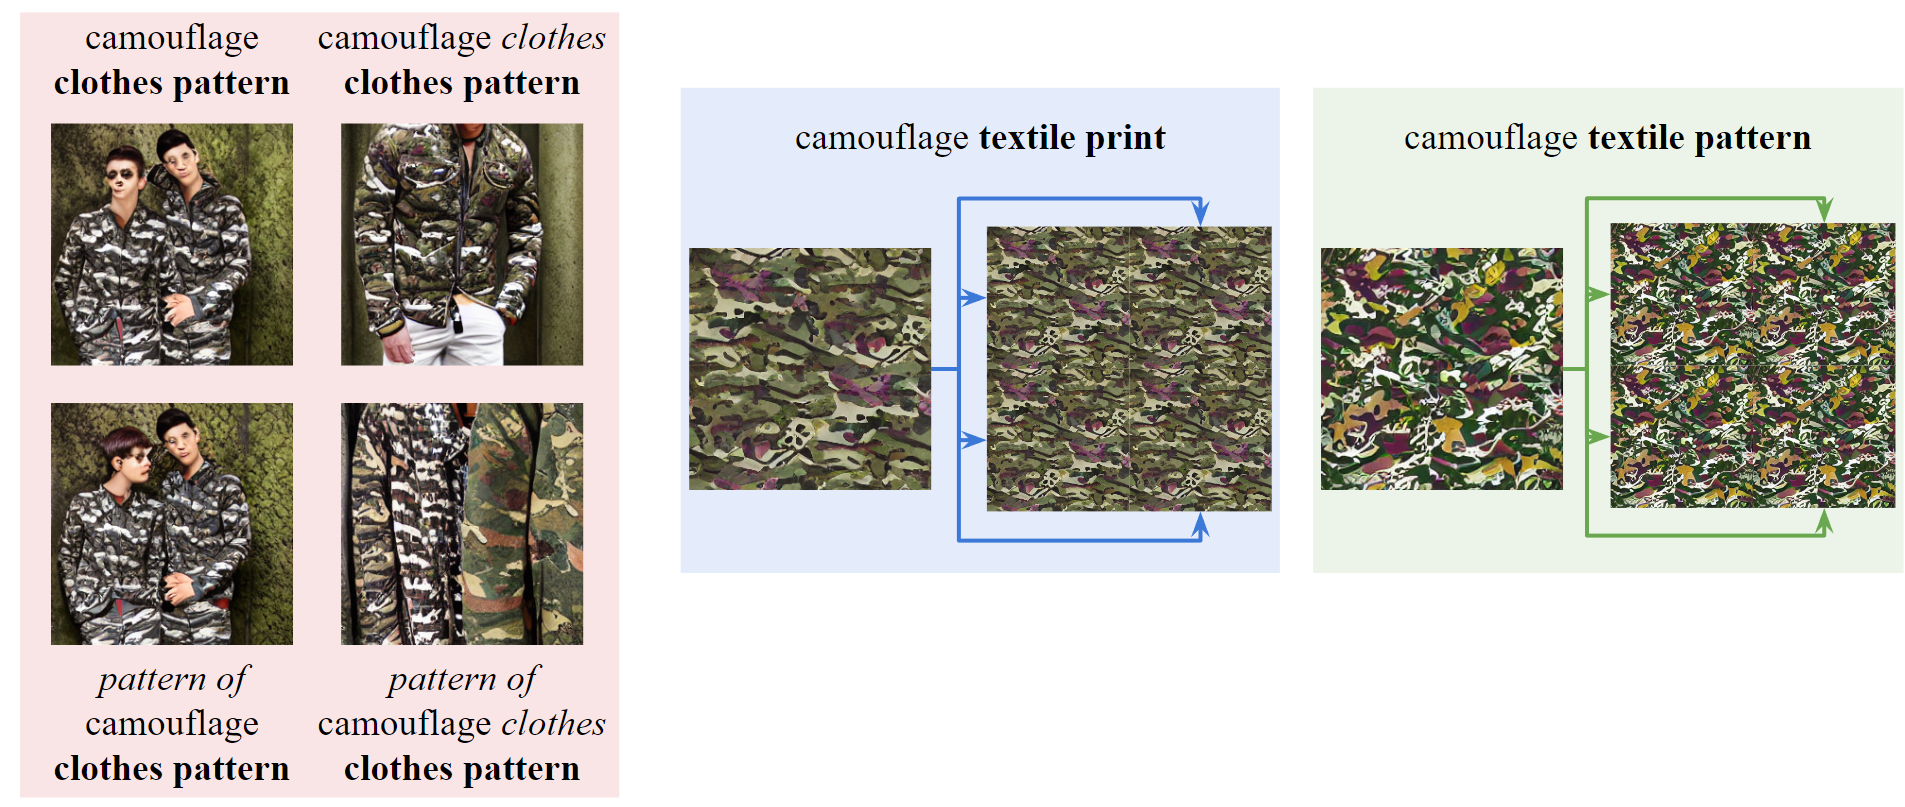
\includegraphics[width=150mm]{figures/clothes_pattern_fails.png}
\caption{``clothes pattern'' extension fails.}
\label{clothes_pattern_fails}
\end{figure}

The obvious problem of this approach is that there is nothing that guarantees that the chosen prompt extension will work as intended, creating a continuous pattern.
For example, the ``clothes pattern'' extension fails on the ``camouflage'' prompt, as shown in the upper-left image of the red part of  Figure~\ref{clothes_pattern_fails}.
This can be explained by the fact that words like ``camouflage'' and ``clothes'' often go together, so the SD model has learned some additional dependencies and creates specific generations like the one we observe.
Adding another ``clothes'' or enhancing the tiling effect with an additional ``pattern of'', as suggested in the example of Figure~\ref{tiling_b}, does not solve the problem.

Even though this particular problem can be solved by choosing another prompt extension like ``textile print'' or ``textile pattern'', as demonstrated in the blue and green parts of Figure~\ref{clothes_pattern_fails}, there is no guarantee that these other extension work for all possible prompts.

\paragraph{TV-loss}
TODO?

\section{Datasets}

In this section, we briefly describe the datasets that have been used during the research and our methods to add clothes to the generated data.

\paragraph{Inria Person}

TODO

\paragraph{Background}

TODO

\section{Evaluation}

In this section, we will briefly introduce the metrics that we are most likely to use for the evasion task.

\paragraph{IoU threshold}
Whether a box predicted by a detector is considered a valid object is decided based on the intersection over union (IoU) score.
In case if there are many overlapping boxes on a test image like in the Inria Dataset that is often used for evaluation, a relatively high IoU threshold of 0.5 is usually chosen.
However, a high threshold value may lead to overestimation of the effectiveness of the attack, so we intend to study different values.

\paragraph{AP} 
TODO 

\paragraph{ASR}
We define Attack Success Rate (ASR) as the ratio between the incorrectly predicted test images to the total number of test images.
An object is considered as correctly identified if the objectiveness score for it is higher than 0,5.
% TODO 

\paragraph{Naturalness}
~\cite{dog_patch_clothes} suggested using subjective evaluation to get a naturalness score of a patch.
For this evaluation, a number of participants is invited to estimate how natural the clothes in question look.
A naturalness evaluation is not difficult to perform since the number of participants should not necessarily be very high---in~\cite{dog_patch_clothes}, it was 24.
% TODO water

TODO describe problems with metrics

\section{Experiments}

In this section, we present the results of the method in different scenarios.
% TODO more about what we analyse 

\subsection{2D Pipeline}

\begin{figure}[htp]
\centering
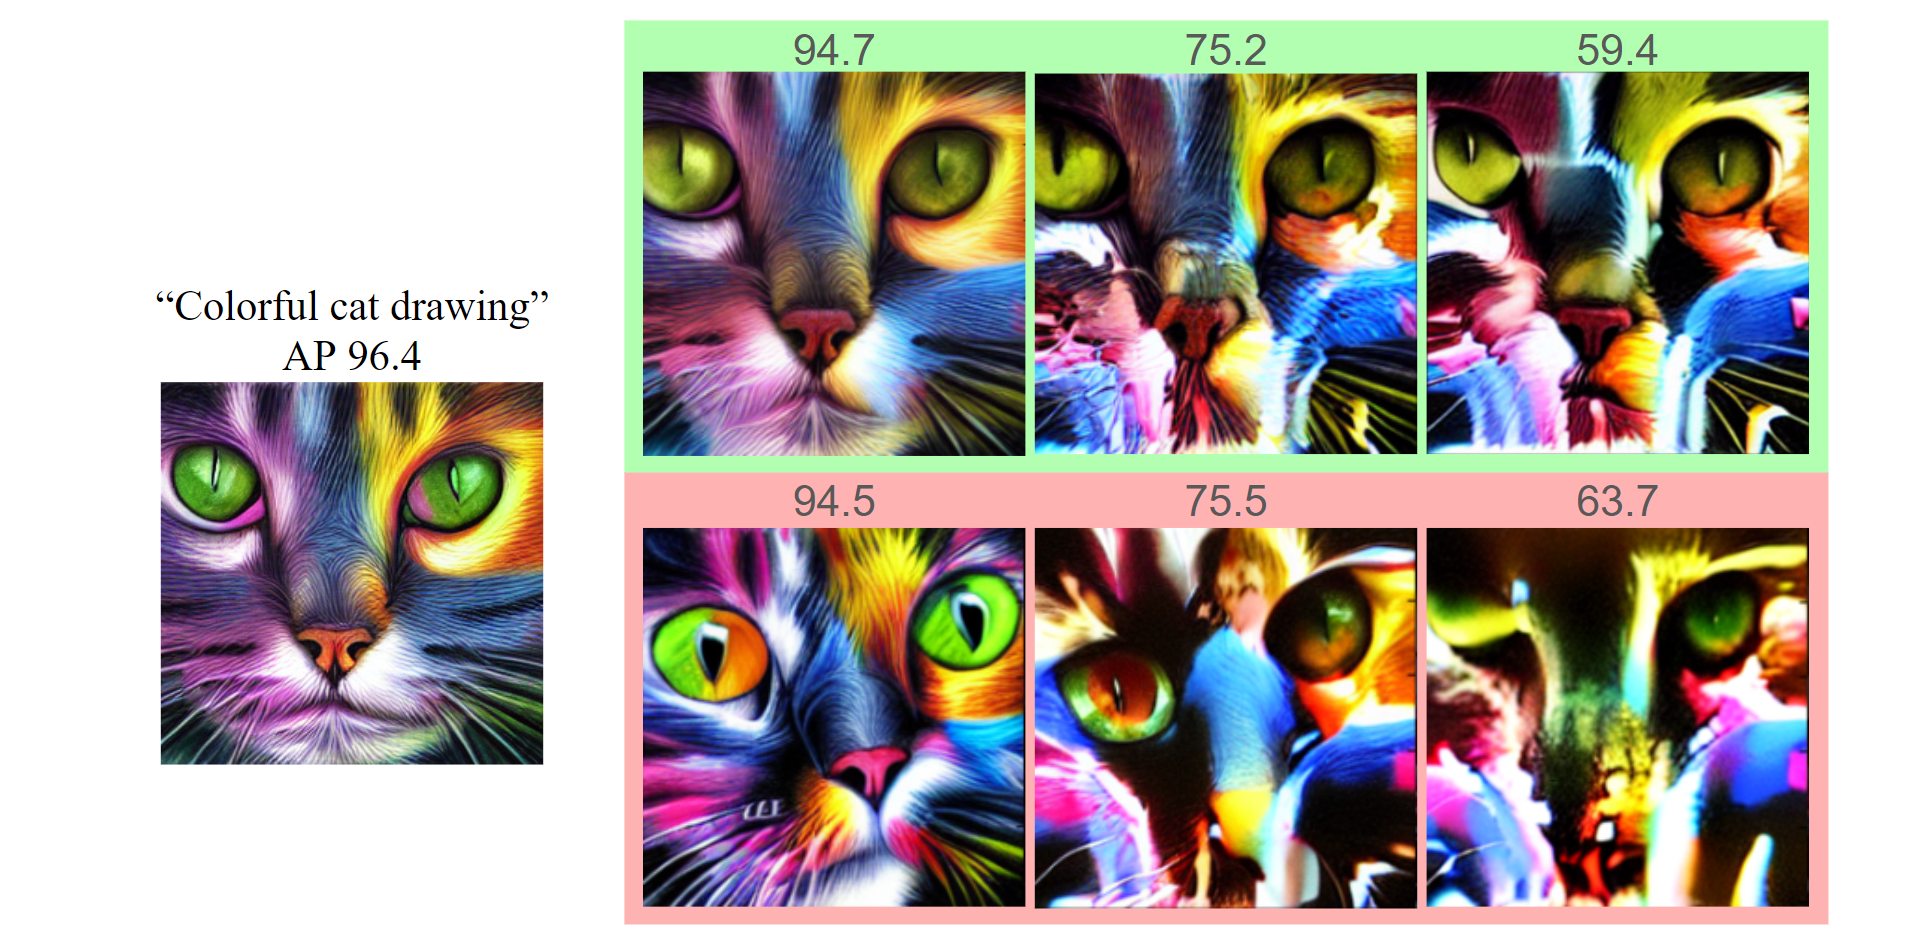
\includegraphics[width=150mm]{figures/2d_res.png}
\caption{Experimental results for 2D pipeline, prompt ``colorful cat drawing''. Only adversarial guidance.}
\label{2d_res}
\end{figure}

Figure~\ref{2d_res} presents results obtained with the 2D pipeline for prompt ``colorful cat drawing'' for the original SD generation on the left and 6 adversarial generations with different schedulers on the right.

The upper green row shows relatively good results: the AP decreases as we trade naturalness of the picture for its effectiveness.
The lower red row is significantly worse: we stray far away from our original generation on the left while achieving similar APs; moreover, the last two generations do not even appear natural.
As a reminder, we also reiterate the reason why we want our adversarial generation to be close to the original image: we want to be able to control our final result, so, instead of just obtaining any image from the ``colorful cat drawing'' space, we want something close to provided image.

The first image in the lower world looks realistic, but has a high AP and is very far away from the original image.
The reason behind this is that the scheduler that was used to create this generation had very high adversarial coefficients in the beginning and low by the end of the generations.
Basically, we just started from a different noise and arrived at another natural image that just happened to be more adversarial.
While optimizing latent as another part of the pipeline is promising in terms of adversarial effectiveness, we would have lost any control as soon as we switched to this method.

\begin{figure}[htp]
\centering
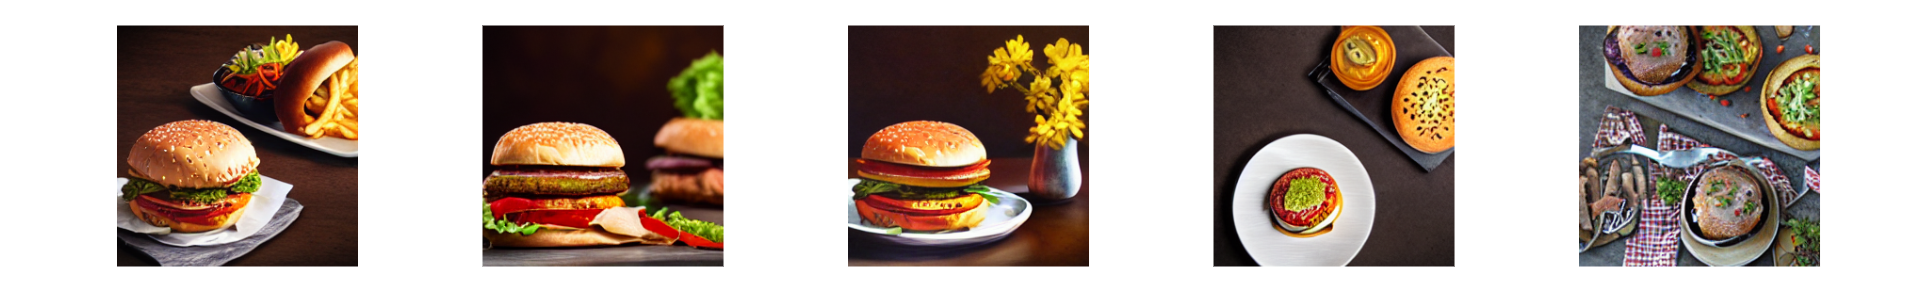
\includegraphics[width=150mm]{figures/hamburger.png}
\caption{``A hamburger on a table'', SD. Different number of steps between 30 and 512.}
\label{hamburger}
\end{figure}

Moreover, more often than not, a random noise that leads to higher adversarial effects also has absolutely unnatural non-adversarial generations.
For example, for the ``a hamburger on a table'' prompt, SD generates very different results depending on the number of steps, as demonstrated in Figure~\ref{hamburger}.
The same generally holds true for all prompts.
It turns out that we can achieve higher adversarial effects if we guide the last generation; however, as we can see, this additional effectiveness comes at the cost of naturalness as well, so we do not look for the best starting latent and rather focus on controlling the generation process to produce something close to the original image.
This also reinforces the theory that appearance constraint guidance is very important for our method.

The major problem of this approach is the fact that the APs are undeniably high, while the naturalness fades away rather swiftly; even more importantly, we are unable to achieve lower APs with this method, and higher coefficients in adversarial schedulers only lead to complete vanishing of naturalness and no decrease in adversarial effectiveness, like in the last generation with AP 63,7.

This is the initial pipeline we used, and it turned out to be so much less effective than the 3D pipeline that examples of the results are only presented in this subsection; the rest of this section is dedicated to the 3D pipeline.

\subsection{Adversarial Guidance}

\begin{figure}[htp]
\centering
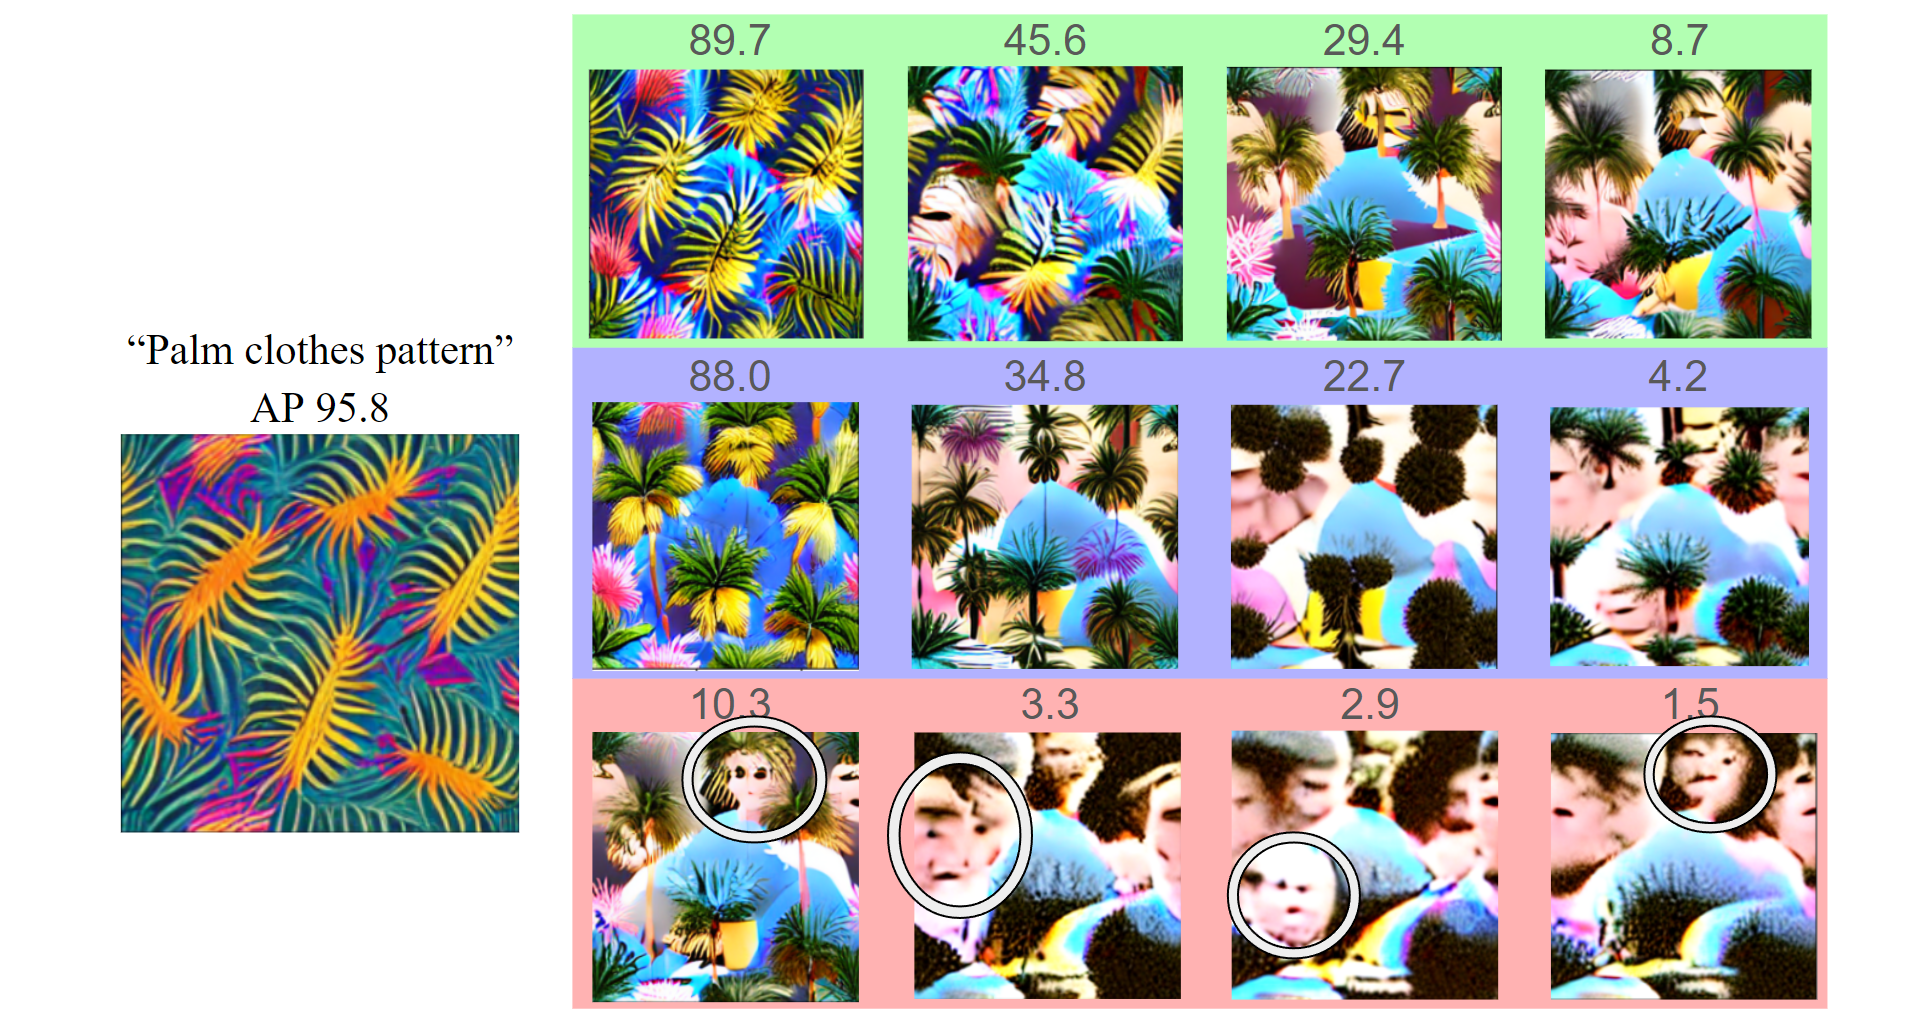
\includegraphics[width=150mm]{figures/3d_res_wo_fix.png}
\caption{Experimental results for the 3D pipeline, prompt ``palm clothes pattern''. Only adversarial guidance.}
\label{3d_wo_fix}
\end{figure}

After switching to the 3D pipeline, we immediately achieve much lower APs, as shown in Figure~\ref{3d_wo_fix} on the example of the ``palm clothes pattern'' prompt adversarial generations for 12 different schedulers. 

The generations on the upper green row are good and follow our expectations: as we apply stronger adversarial guidance coefficients, we go further away from the original non-adversarial generation on the right but also avoid detection better.
Even though the last two images in this row do not resemble the original generation, we at least still observe ``palms'' in the resulting patches. 

For the second blue row, while the adversarial effects are similar to the upper row, the generations are significantly worse: the first two have APs that are disproportionately large compared to how close they are to the original picture, and the last two are even more far away from the original compared to the corresponding images above and do not even seem to follow the prompt very well either. 
The scheduler used to generate the first image had adversarial coefficients that were high in the beginning and very low in the end, so, just like in similar experiments with the 2D pipeline, we obtain an image from the same space of ``palm clothes pattern'' generations but as if we started from another noise. 

The last red row shows a common artifact that appears on the generations with low APs, that is, with very strong adversarial schedulers. 
First of all, the three last generations can be labeled as failures: they are neither natural nor even comply with the prompt conditioning. 
The artifact, people's faces, is a common problem not just in this method, but in detector evasion in general~\cite{texture}.
As a physical explanation, one might think of it as if after a person puts on the adversarial clothes, the model starts seeing many people in their silhouette and loses the big figure of the person themself.
This artifact almost always accompanies low APs, and it is difficult to get rid of it, but appearance restoration does somewhat alleviate this problem.

% TODO 

\subsection{Appearance Restoration}

\begin{figure}[htp]
\subfloat[``Palm clothes pattern''.]{
  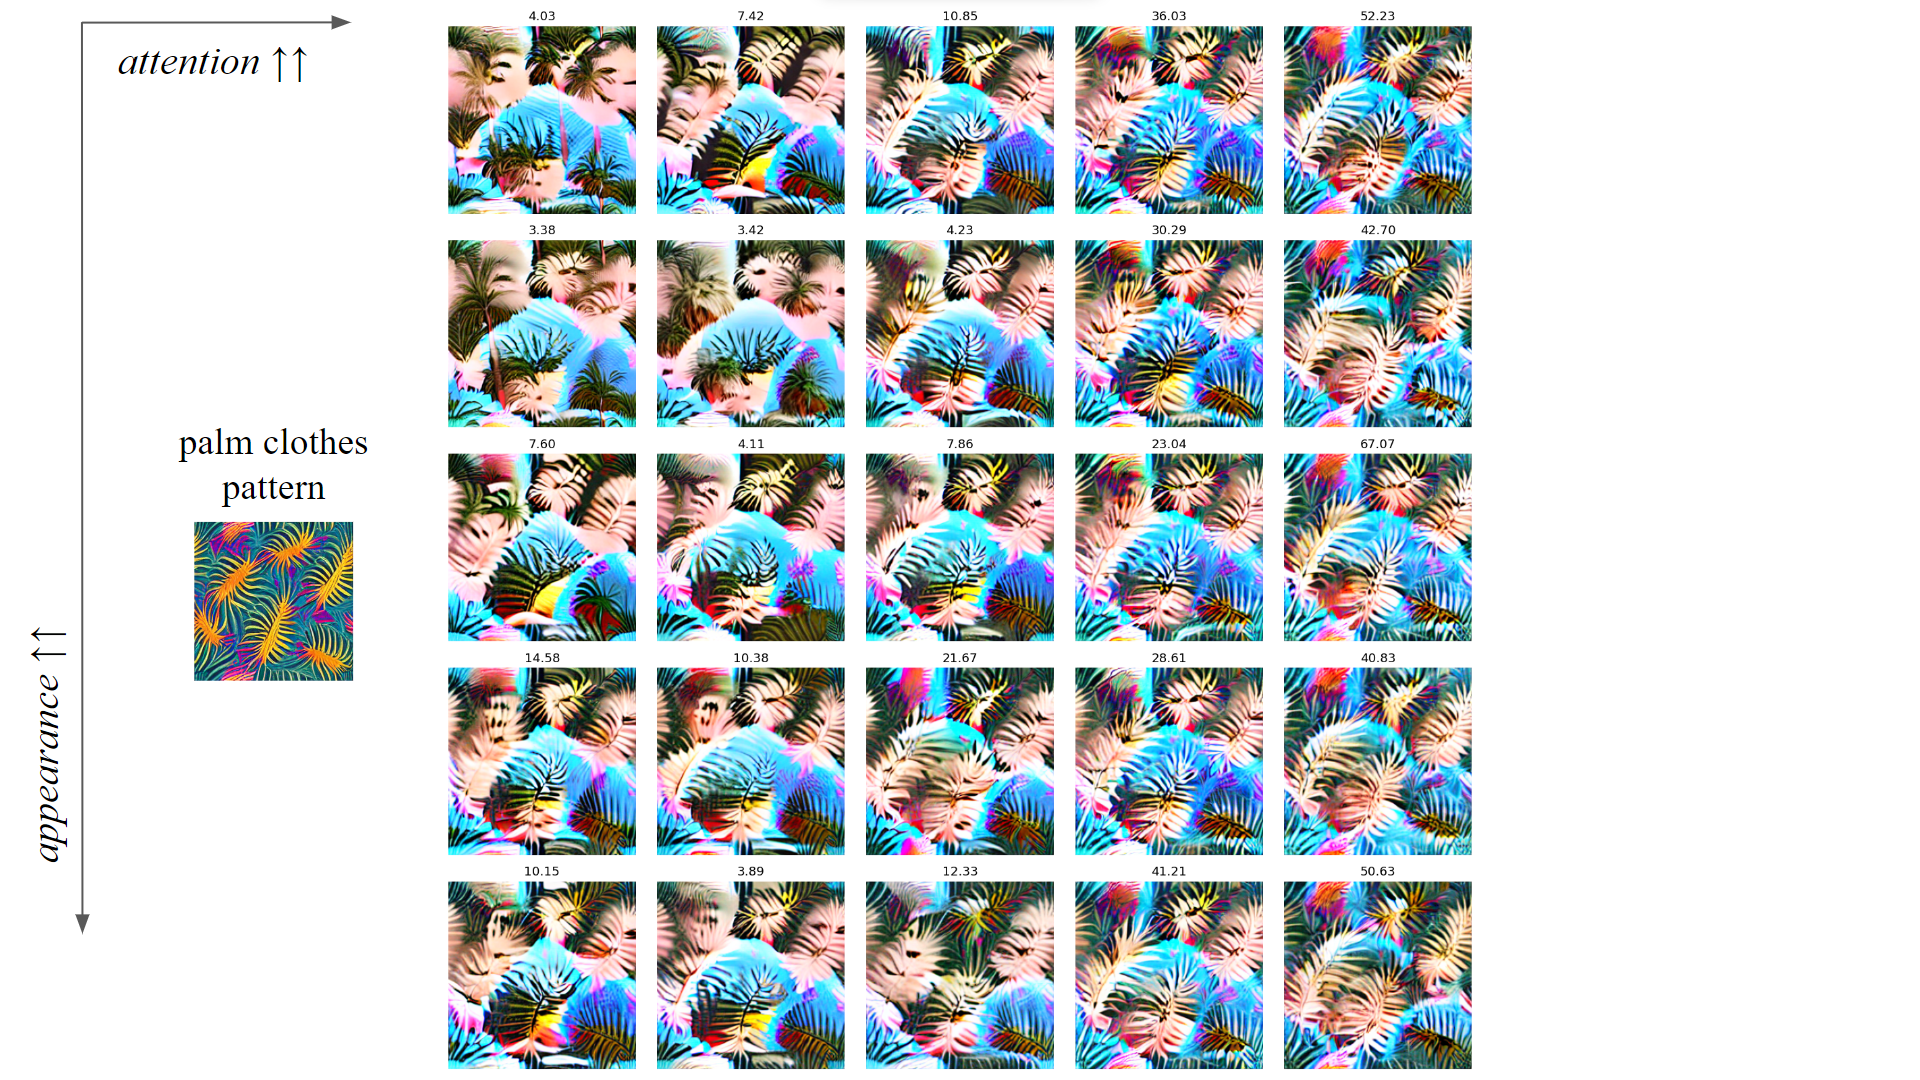
\includegraphics[clip, width=\columnwidth]{figures/fix_palm.png}\label{fix_palm}
}\hfill
\subfloat[``Space clothes pattern''.]{
  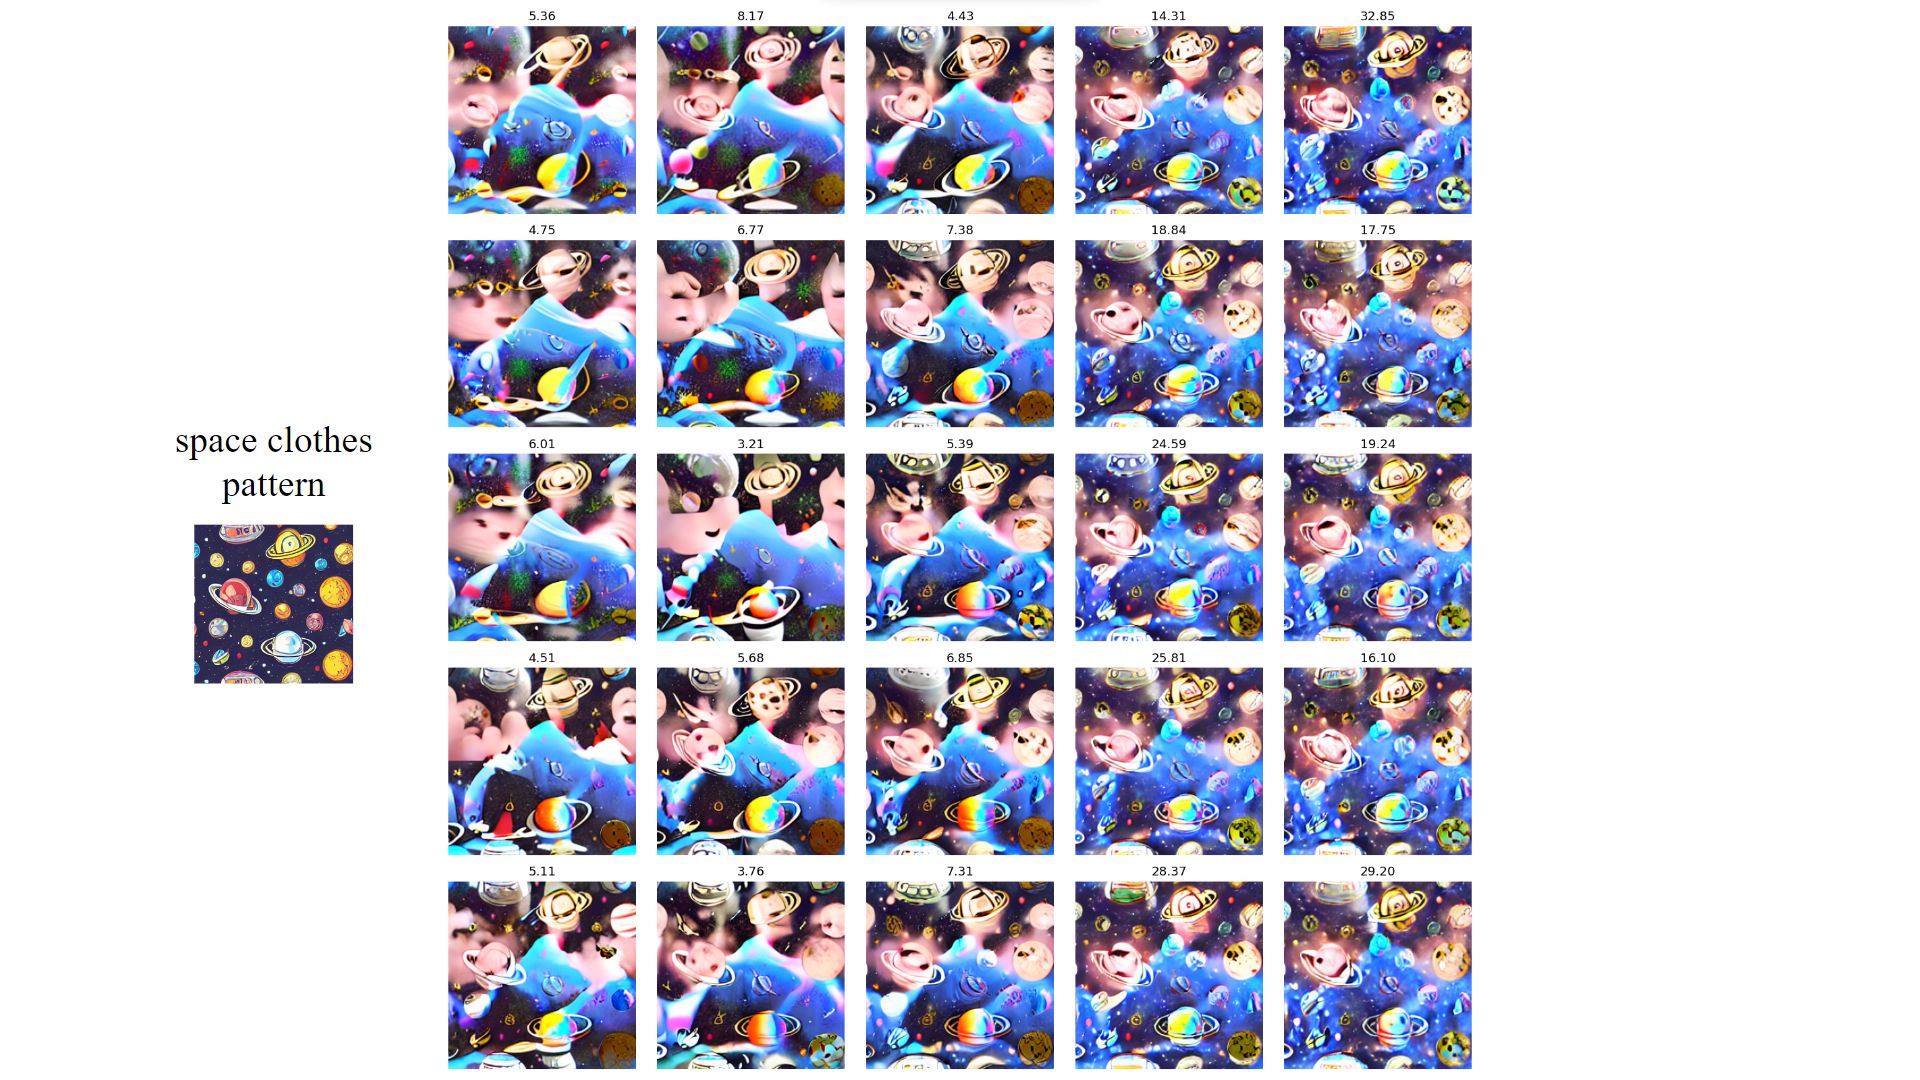
\includegraphics[clip, width=\columnwidth]{figures/fix_space.png}\label{fix_space}
}
\caption{Generations for the same adversarial scheduler with different strength of $s^{at}$ and $s^{ap}$ coefficients.}\label{fix_ex}
\end{figure}

Figure~\ref{fix_ex} shows how the trade-off between adversarial effectiveness and resemblance to the original image by varying attention and appearance constraint coefficients for two prompts, ``palm clothes pattern'' (Figure~\ref{fix_palm}) and ``space clothes pattern'' (Figure~\ref{fix_space}).

In the left part of both figures, we can see the non-adversarial versions for the prompts.

Appearance constraint coefficient $s^{ap}$ increases along the $y$ axis (top to bottom direction), while the self-attention constraint coefficient $s^{at}$ increases along the $x$ axis (left to right direction), so the last images in the last rows are the closest to their respective non-adversarial images, but also have the lowest adversarial effects.
While the resemblance to the non-adversarial pictures increases along both axes, we can see that self-attention constraint is indeed more effective for the same coefficients.

Sadly, we also notice that luck plays a visible part in the results since the AP does not change consistently.
However, considering the fact that we only generated the images for 256 steps and used a weak SD model but managed to obtain good APs nevertheless, the method looks very promising.
The AP is calculated in the digital world scenarios, but the patches are likely to be effective in the real physical world if the AP is at least lower than 7, and both prompts have relatively natural generations that satisfy that requirement. 

\subsection{Different Prompts}

TODO maybe best results for around 5 random prompts, and also with different prompt extensions

\subsection{Real Images}

TODO we can give the model real images, use ddim inversion to obtain latents and work with them (or perhaps phantom trajectories like in self-guidance paper?)

\subsection{Physical Results}

\paragraph{Patches}

\begin{figure}[htp]
\subfloat[``Space clothes pattern'' prompt, AP 12.]{
  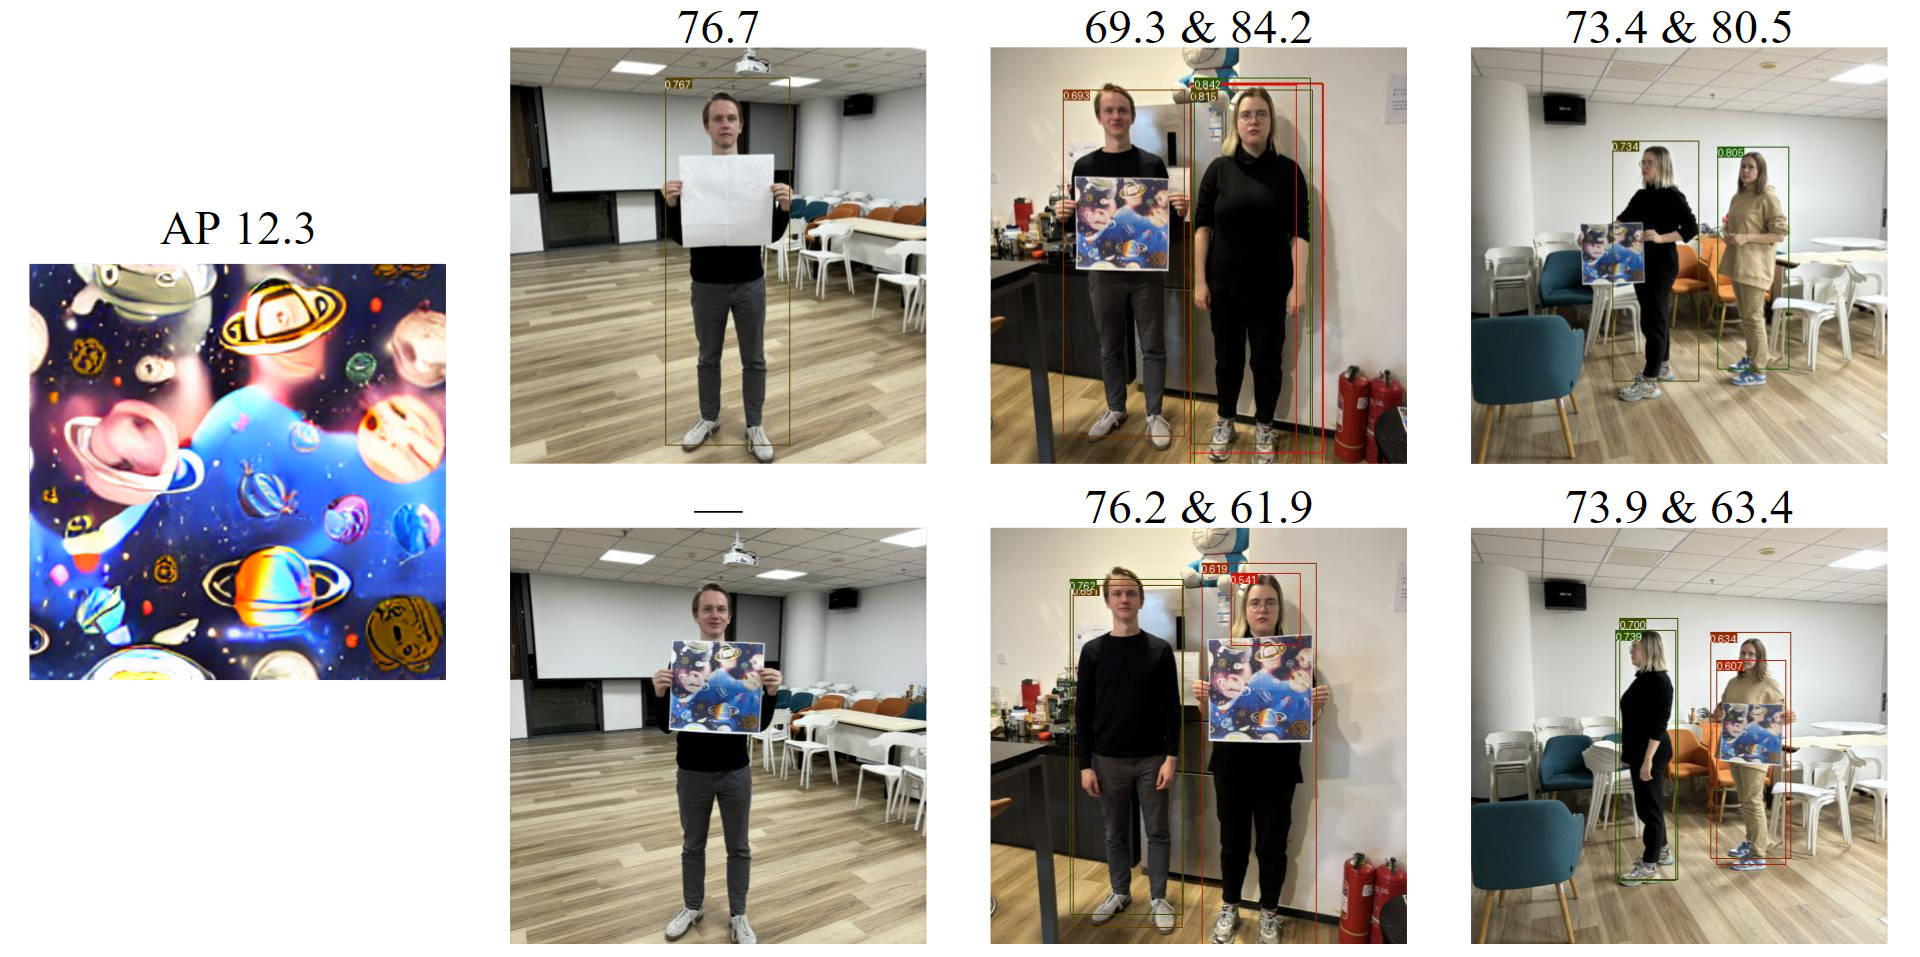
\includegraphics[clip, width=0.9\textwidth]{figures/phys_patch_space1.png}\label{physical_patch_space1}
}\hfill
\subfloat[``Space clothes pattern'' prompt, AP 4.]{
  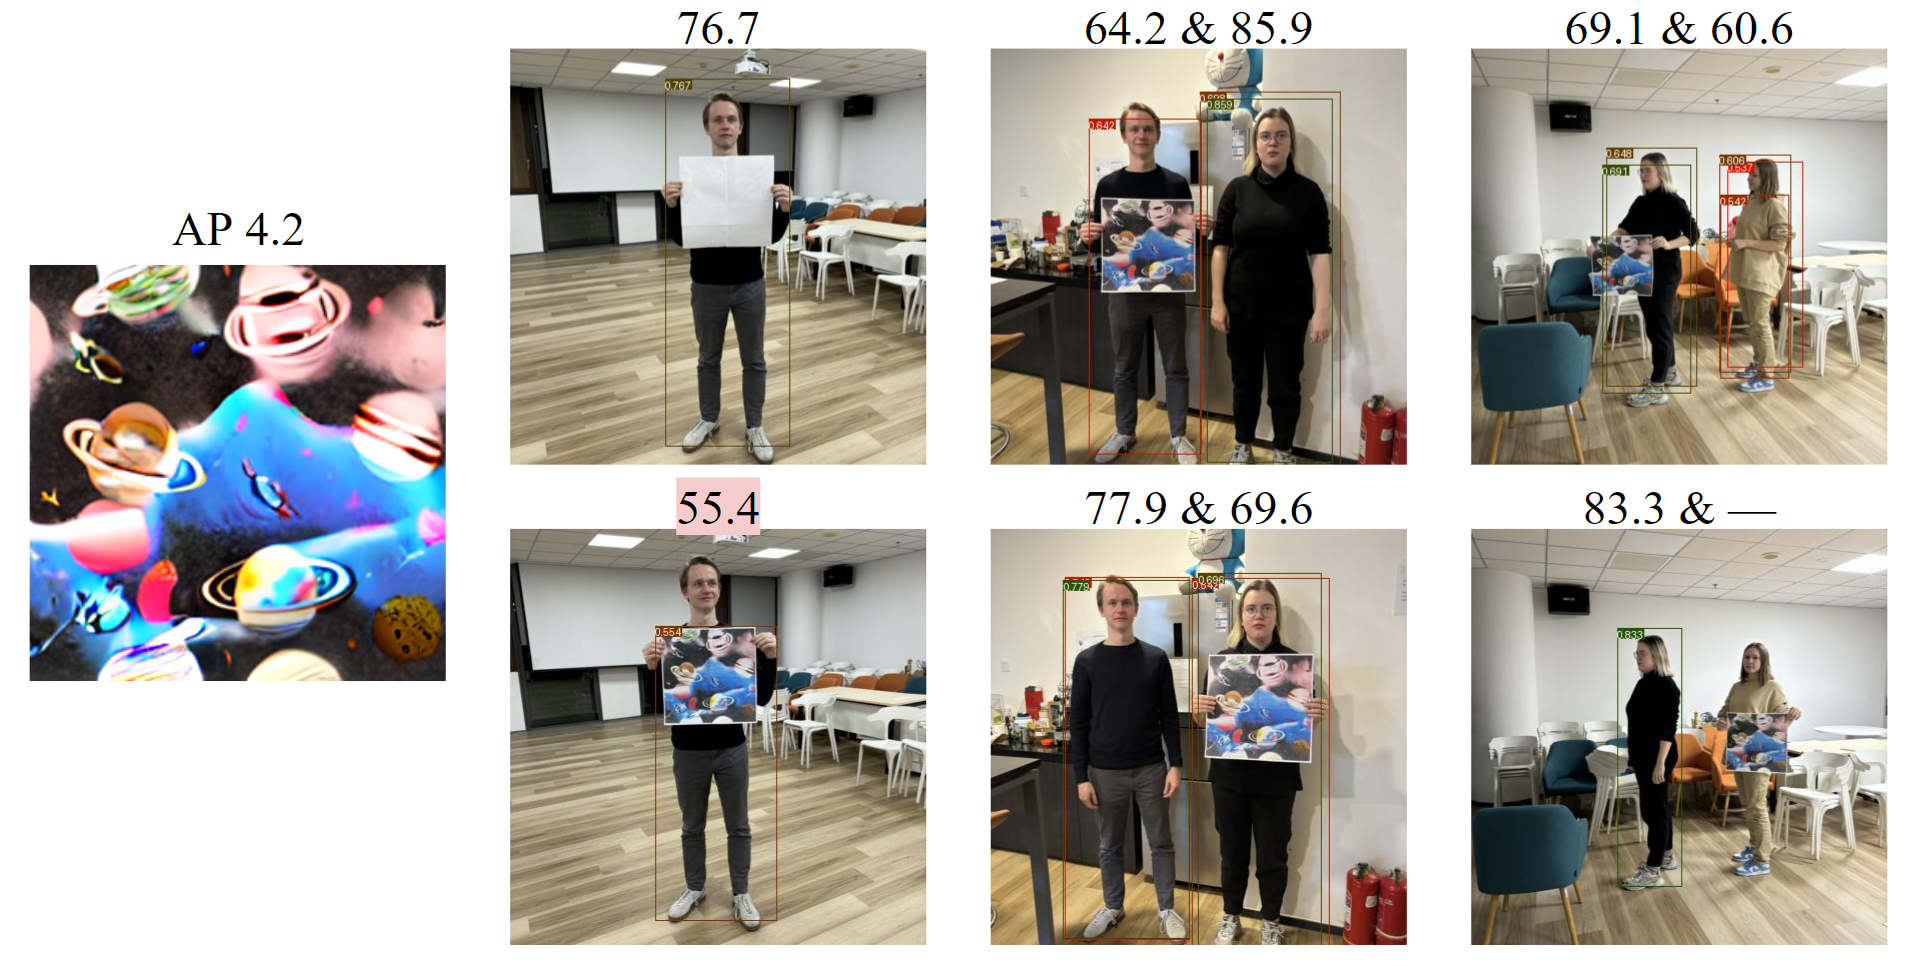
\includegraphics[clip, width=0.9\textwidth]{figures/phys_patch_space2.png}\label{physical_patch_space2}
}\hfill
\subfloat[``Flower clothes pattern'' prompt, AP 57.]{
  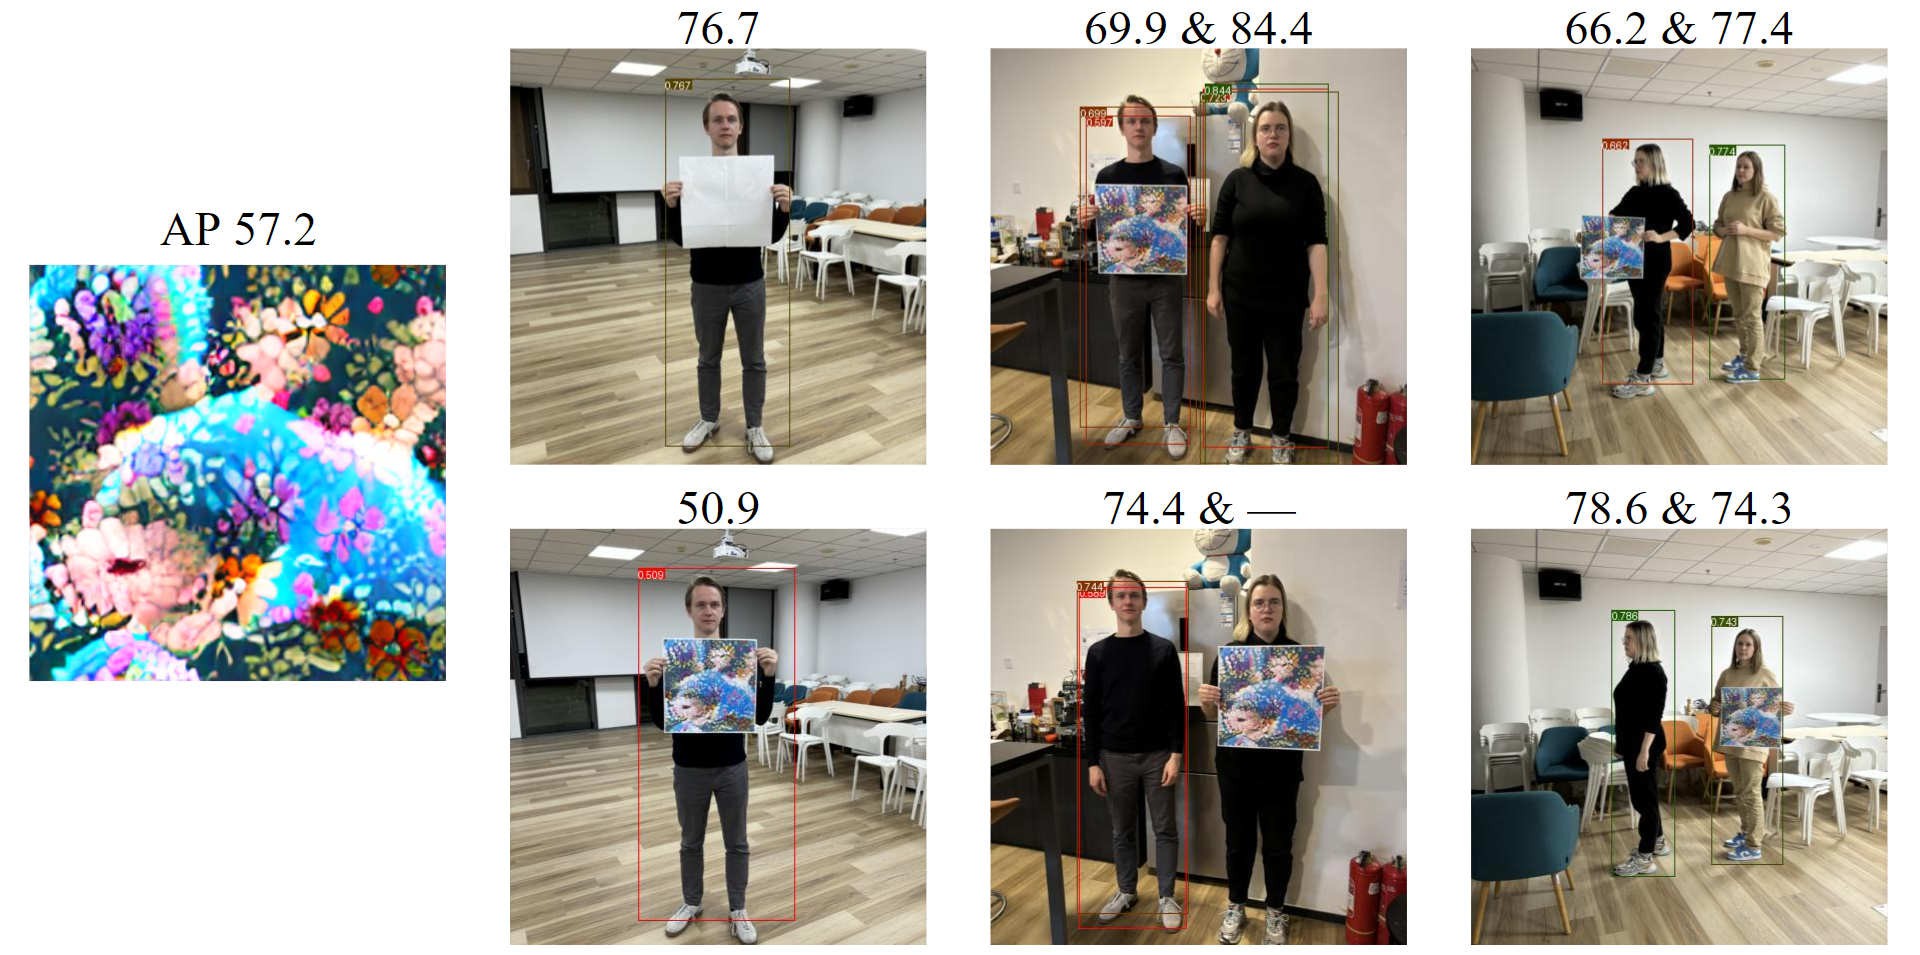
\includegraphics[clip, width=0.9\textwidth]{figures/phys_patch_flower.png}\label{physical_patch_flower}
}
\caption{Physical results with generations as patches trained with the 3D pipeline.}\label{physical_patches}
\end{figure}
 
Evaluation of physical results is rather challenging, mainly because printing actual clothes, taking videos with them, and then manually labelling all the data is very time-consuming and expensive.
Firstly, we need to ensure that the generated patterns actually work by, for example, only printing them as patches and checking their effectiveness in several settings. 
Examples of this approach can be found in Figure~\ref{physical_patches}.

TODO desc

\paragraph{Clothes}

TODO?

\section{Comparison Against Baseline Methods}

TODO for this, we need to switch to yolo3 


% \section{数学符号}

% 中文论文的数学符号默认遵循 GB/T 3102.11—1993《物理科学和技术中使用的数学符号》
% \footnote{原 GB 3102.11—1993,自 2017 年 3 月 23 日起,该标准转为推荐性标准。}。
% 该标准参照采纳 ISO 31-11:1992 \footnote{目前已更新为 ISO 80000-2:2019。},
% 但是与 \TeX{} 默认的美国数学学会(AMS)的符号习惯有所区别。
% 具体地来说主要有以下差异:
% \begin{enumerate}
%   \item 大写希腊字母默认为斜体,如
%     \begin{equation*}
%       \Gamma \Delta \Theta \Lambda \Xi \Pi \Sigma \Upsilon \Phi \Psi \Omega.
%     \end{equation*}
%     注意有限增量符号 $\increment$ 固定使用正体,模板提供了 \cs{increment} 命令。
%   \item 小于等于号和大于等于号使用倾斜的字形 $\le$、$\ge$。
%   \item 积分号使用正体,比如 $\int$、$\oint$。
%   \item
%     偏微分符号 $\partial$ 使用正体。
%   \item
%     省略号 \cs{dots} 按照中文的习惯固定居中,比如
%     \begin{equation*}
%       1, 2, \dots, n \quad 1 + 2 + \dots + n.
%     \end{equation*}
%   \item
%     实部 $\Re$ 和虚部 $\Im$ 的字体使用罗马体。
% \end{enumerate}

% 以上数学符号样式的差异可以在模板中统一设置。
% 另外国标还有一些与 AMS 不同的符号使用习惯,需要用户在写作时进行处理:
% \begin{enumerate}
%   \item 数学常数和特殊函数名用正体,如
%     \begin{equation*}
%       \uppi = 3.14\dots; \quad
%       \symup{i}^2 = -1; \quad
%       \symup{e} = \lim_{n \to \infty} \left( 1 + \frac{1}{n} \right)^n.
%     \end{equation*}
%   \item 微分号使用正体,比如 $\dif y / \dif x$。
%   \item 向量、矩阵和张量用粗斜体(\cs{symbf}),如 $\symbf{x}$、$\symbf{\Sigma}$、$\symbfsf{T}$。
%   \item 自然对数用 $\ln x$ 不用 $\log x$。
% \end{enumerate}


% 英文论文的数学符号使用 \TeX{} 默认的样式。
% 如果有必要,也可以通过设置 \verb|math-style| 选择数学符号样式。

% 关于量和单位推荐使用
% \href{http://mirrors.ctan.org/macros/latex/contrib/siunitx/siunitx.pdf}{\pkg{siunitx}}
% 宏包,
% 可以方便地处理希腊字母以及数字与单位之间的空白,
% 比如:
% \SI{6.4e6}{m},
% \SI{9}{\micro\meter},
% \si{kg.m.s^{-1}},
% \SIrange{10}{20}{\degreeCelsius}。



% \section{数学公式}

% 数学公式可以使用 \env{equation} 和 \env{equation*} 环境。
% 注意数学公式的引用应前后带括号,通常使用 \cs{eqref} 命令,比如式\eqref{eq:example}。
% \begin{equation}
%   \frac{1}{2 \uppi \symup{i}} \int_\gamma f = \sum_{k=1}^m n(\gamma; a_k) \mathscr{R}(f; a_k).
%   \label{eq:example}
% \end{equation}

% 多行公式尽可能在“=”处对齐,推荐使用 \env{align} 环境。
% \begin{align}
%   a & = b + c + d + e \\
%     & = f + g
% \end{align}



% \section{数学定理}

% 定理环境的格式可以使用 \pkg{amsthm} 或者 \pkg{ntheorem} 宏包配置。
% 用户在导言区载入这两者之一后,模板会自动配置 \env{thoerem}、\env{proof} 等环境。

% \begin{theorem}[Lindeberg--Lévy 中心极限定理]
%   设随机变量 $X_1, X_2, \dots, X_n$ 独立同分布, 且具有期望 $\mu$ 和有限的方差 $\sigma^2 \ne 0$,
%   记 $\bar{X}_n = \frac{1}{n} \sum_{i+1}^n X_i$,则
%   \begin{equation}
%     \lim_{n \to \infty} P \left(\frac{\sqrt{n} \left( \bar{X}_n - \mu \right)}{\sigma} \le z \right) = \Phi(z),
%   \end{equation}
%   其中 $\Phi(z)$ 是标准正态分布的分布函数。
% \end{theorem}
% \begin{proof}
%   Trivial.
% \end{proof}

% 同时模板还提供了 \env{assumption}、\env{definition}、\env{proposition}、
% \env{lemma}、\env{theorem}、\env{axiom}、\env{corollary}、\env{exercise}、
% \env{example}、\env{remar}、\env{problem}、\env{conjecture} 这些相关的环境。

% !TeX root = ../thuthesis-example.tex

\chapter{CONCLUSION}

\section{Work and Contribution}

TODO (\cite{routh2009anatomical})

\section{Future Work}

TODO

% 模板支持 BibTeX 和 BibLaTeX 两种方式处理参考文献。
% 下文主要介绍 BibTeX 配合 \pkg{natbib} 宏包的主要使用方法。


% \section{顺序编码制}

% 在顺序编码制下,默认的 \cs{cite} 命令同 \cs{citep} 一样,序号置于方括号中,
% 引文页码会放在括号外。
% 统一处引用的连续序号会自动用短横线连接。

% \thusetup{
%   cite-style = super,
% }
% \noindent
% \begin{tabular}{l@{\quad$\Rightarrow$\quad}l}
%   \verb|\cite{zhangkun1994}|               & \cite{zhangkun1994}               \\
%   \verb|\citet{zhangkun1994}|              & \citet{zhangkun1994}              \\
%   \verb|\citep{zhangkun1994}|              & \citep{zhangkun1994}              \\
%   \verb|\cite[42]{zhangkun1994}|           & \cite[42]{zhangkun1994}           \\
%   \verb|\cite{zhangkun1994,zhukezhen1973}| & \cite{zhangkun1994,zhukezhen1973} \\
% \end{tabular}


% 也可以取消上标格式,将数字序号作为文字的一部分。
% 建议全文统一使用相同的格式。

% \thusetup{
%   cite-style = inline,
% }
% \noindent
% \begin{tabular}{l@{\quad$\Rightarrow$\quad}l}
%   \verb|\cite{zhangkun1994}|               & \cite{zhangkun1994}               \\
%   \verb|\citet{zhangkun1994}|              & \citet{zhangkun1994}              \\
%   \verb|\citep{zhangkun1994}|              & \citep{zhangkun1994}              \\
%   \verb|\cite[42]{zhangkun1994}|           & \cite[42]{zhangkun1994}           \\
%   \verb|\cite{zhangkun1994,zhukezhen1973}| & \cite{zhangkun1994,zhukezhen1973} \\
% \end{tabular}



% \section{著者-出版年制}

% 著者-出版年制下的 \cs{cite} 跟 \cs{citet} 一样。

% \thusetup{
%   cite-style = author-year,
% }
% \noindent
% \begin{tabular}{@{}l@{$\Rightarrow$}l@{}}
%   \verb|\cite{zhangkun1994}|                & \cite{zhangkun1994}                \\
%   \verb|\citet{zhangkun1994}|               & \citet{zhangkun1994}               \\
%   \verb|\citep{zhangkun1994}|               & \citep{zhangkun1994}               \\
%   \verb|\cite[42]{zhangkun1994}|            & \cite[42]{zhangkun1994}            \\
%   \verb|\citep{zhangkun1994,zhukezhen1973}| & \citep{zhangkun1994,zhukezhen1973} \\
% \end{tabular}

% \vskip 2ex
% \thusetup{
%   cite-style = super,
% }
% 注意,引文参考文献的每条都要在正文中标注
% \cite{zhangkun1994,zhukezhen1973,dupont1974bone,zhengkaiqing1987,%
%   jiangxizhou1980,jianduju1994,merkt1995rotational,mellinger1996laser,%
%   bixon1996dynamics,mahui1995,carlson1981two,taylor1983scanning,%
%   taylor1981study,shimizu1983laser,atkinson1982experimental,%
%   kusch1975perturbations,guangxi1993,huosini1989guwu,wangfuzhi1865songlun,%
%   zhaoyaodong1998xinshidai,biaozhunhua2002tushu,chubanzhuanye2004,%
%   who1970factors,peebles2001probability,baishunong1998zhiwu,%
%   weinstein1974pathogenic,hanjiren1985lun,dizhi1936dizhi,%
%   tushuguan1957tushuguanxue,aaas1883science,fugang2000fengsha,%
%   xiaoyu2001chubanye,oclc2000about,scitor2000project%
% }。



% 其他部分
\backmatter

% 参考文献
\bibliography{ref/refs}  % 参考文献使用 BibTeX 编译
% \printbibliography       % 参考文献使用 BibLaTeX 编译

% 附录
% 本科生需要将附录放到声明之后,个人简历之前
\appendix
% % !TeX root = ../thuthesis-example.tex

\begin{survey}
\label{cha:survey}

\title{Title of the Survey}
\maketitle


\tableofcontents


本科生的外文资料调研阅读报告。


\section{Figures and Tables}

\subsection{Figures}

An example figure in appendix (Figure~\ref{fig:appendix-survey-figure}).

\begin{figure}
  \centering
  \includegraphics[width=0.6\linewidth]{example-image-a.pdf}
  \caption{Example figure in appendix}
  \label{fig:appendix-survey-figure}
\end{figure}


\subsection{Tables}

An example table in appendix (Table~\ref{tab:appendix-survey-table}).

\begin{table}
  \centering
  \caption{Example table in appendix}
  \begin{tabular}{ll}
    \toprule
    File name       & Description                                         \\
    \midrule
    thuthesis.dtx   & The source file including documentaion and comments \\
    thuthesis.cls   & The template file                                   \\
    thuthesis-*.bst & BibTeX styles                                       \\
    thuthesis-*.bbx & BibLaTeX styles for bibliographies                  \\
    thuthesis-*.cbx & BibLaTeX styles for citations                       \\
    \bottomrule
  \end{tabular}
  \label{tab:appendix-survey-table}
\end{table}


\section{Equations}

An example equation in appendix (Equation~\eqref{eq:appendix-survey-equation}).
\begin{equation}
  \frac{1}{2 \uppi \symup{i}} \int_\gamma f = \sum_{k=1}^m n(\gamma; a_k) \mathscr{R}(f; a_k)
  \label{eq:appendix-survey-equation}
\end{equation}


\section{Citations}

Example citations in appendix.
\cite{abrahams99tex}
\cite{salomon1995advanced}
\cite{abrahams99tex,salomon1995advanced}


\bibliographystyle{unsrtnat}
\bibliography{ref/appendix}

\end{survey}
       % 本科生:外文资料的调研阅读报告
% % !TeX root = ../thuthesis-example.tex

\begin{translation}
\label{cha:translation}

\title{书面翻译题目}
\maketitle

\tableofcontents


本科生的外文资料书面翻译。


\section{图表示例}

\subsection{图}

附录中的图片示例(图~\ref{fig:appendix-translation-figure})。

\begin{figure}
  \centering
  \includegraphics[width=0.6\linewidth]{example-image-a.pdf}
  \caption{附录中的图片示例}
  \label{fig:appendix-translation-figure}
\end{figure}


\subsection{表格}

附录中的表格示例(表~\ref{tab:appendix-translation-table})。

\begin{table}
  \centering
  \caption{附录中的表格示例}
  \begin{tabular}{ll}
    \toprule
    文件名          & 描述                         \\
    \midrule
    thuthesis.dtx   & 模板的源文件,包括文档和注释 \\
    thuthesis.cls   & 模板文件                     \\
    thuthesis-*.bst & BibTeX 参考文献表样式文件    \\
    thuthesis-*.bbx & BibLaTeX 参考文献表样式文件  \\
    thuthesis-*.cbx & BibLaTeX 引用样式文件        \\
    \bottomrule
  \end{tabular}
  \label{tab:appendix-translation-table}
\end{table}


\section{数学公式}

附录中的数学公式示例(公式\eqref{eq:appendix-translation-equation})。
\begin{equation}
  \frac{1}{2 \uppi \symup{i}} \int_\gamma f = \sum_{k=1}^m n(\gamma; a_k) \mathscr{R}(f; a_k)
  \label{eq:appendix-translation-equation}
\end{equation}


\section{文献引用}

文献引用示例\cite{abrahams99tex}。


\appendix

\section{附录}

附录的内容。


% 书面翻译的参考文献
\bibliographystyle{unsrtnat}
\bibliography{ref/appendix}

% 书面翻译对应的原文索引
\begin{translation-index}
  \nocite{salomon1995advanced}
  \bibliographystyle{unsrtnat}
  \bibliography{ref/appendix}
\end{translation-index}

\end{translation}
  % 本科生:外文资料的书面翻译
% % !TeX root = ../thuthesis-example.tex

\chapter{补充内容}

附录是与论文内容密切相关、但编入正文又影响整篇论文编排的条理和逻辑性的资料,例如某些重要的数据表格、计算程序、统计表等,是论文主体的补充内容,可根据需要设置。

附录中的图、表、数学表达式、参考文献等另行编序号,与正文分开,一律用阿拉伯数字编码,
但在数码前冠以附录的序号,例如“图~\ref{fig:appendix-figure}”,
“表~\ref{tab:appendix-table}”,“式\eqref{eq:appendix-equation}”等。


\section{插图}

% 附录中的插图示例(图~\ref{fig:appendix-figure})。

\begin{figure}
  \centering
  \includegraphics[width=0.6\linewidth]{example-image-a.pdf}
  \caption{附录中的图片示例}
  \label{fig:appendix-figure}
\end{figure}


\section{表格}

% 附录中的表格示例(表~\ref{tab:appendix-table})。

\begin{table}
  \centering
  \caption{附录中的表格示例}
  \begin{tabular}{ll}
    \toprule
    文件名          & 描述                         \\
    \midrule
    thuthesis.dtx   & 模板的源文件,包括文档和注释 \\
    thuthesis.cls   & 模板文件                     \\
    thuthesis-*.bst & BibTeX 参考文献表样式文件    \\
    thuthesis-*.bbx & BibLaTeX 参考文献表样式文件  \\
    thuthesis-*.cbx & BibLaTeX 引用样式文件        \\
    \bottomrule
  \end{tabular}
  \label{tab:appendix-table}
\end{table}


\section{数学表达式}

% 附录中的数学表达式示例(式\eqref{eq:appendix-equation})。
\begin{equation}
  \frac{1}{2 \uppi \symup{i}} \int_\gamma f = \sum_{k=1}^m n(\gamma; a_k) \mathscr{R}(f; a_k)
  \label{eq:appendix-equation}
\end{equation}


\section{参考文献}

附录中的参考文献示例(\cite{carlson1981two} 和 \cite{carlson1981two,taylor1983scanning,taylor1981study})。

\printbibliography


% 致谢
% !TeX root = ../thuthesis-example.tex

\begin{acknowledgements}
  I would like to thank my supervisor, Associate Professor Hu Xiaolin, for his guidance and exceptional ability to motivate students.

  This research was guided by Hu Zhanhao, without whom I would not have known how to start working in the area. 
  His close ex-colleagues, other members of our laboratory, Zhang Wei and TODO, also gave priceless advice on multiple occasions in both technical and research directions.

  I would also like to extend my gratitude to all the students in our laboratory for their enthusiastic help and support in weekly meetings and outside of them.

  The GPU resources were provided by the laboratory under Associate Professor Hu's supervision. 
  The experiments will be performed on the computational resources provided by the IDG/McGovern Institute for Brain Research at Tsinghua University.

\end{acknowledgements}


% 声明
\statement
% 将签字扫描后的声明文件 scan-statement.pdf 替换原始页面
% \statement[file=scan-statement.pdf]
% 本科生编译生成的声明页默认不加页脚,插入扫描版时再补上;
% 研究生编译生成时有页眉页脚,插入扫描版时不再重复。
% 也可以手动控制是否加页眉页脚
% \statement[page-style=empty]
% \statement[file=scan-statement.pdf, page-style=plain]

% 个人简历、在学期间完成的相关学术成果
% 本科生可以附个人简历,也可以不附个人简历
% !TeX root = ../thuthesis-example.tex

\begin{resume}

  \section*{Education}

  2022 --- 2024: \textbf{Tsinghua University}, Computer Science and Technology department, Master’s Program ``Advanced Computing Program''.
  Supervisor --- Associate Professor X. Hu, thesis on physical adversarial attacks.

  2018 --- 2022: \textbf{National Research University Higher School of Economics}, Faculty of Computer Science, Bachelor’s Program ``Applied Mathematics and Information Science''.
  Supervisor --- Associate Professor M. Rakhuba, thesis on theoretical ML. 
  Minor in Bioinformatics.

  \section*{Work Experience}
  2022 --- 2024: \textbf{Tsinghua} Research Intern in the Tsinghua Laboratory of Brain and Intelligence.

  2021 --- 2024: \textbf{HSE, Moscow}: Teaching Assistant to Researcher E. Lobacheva.
  
  2021 --- 2022: \textbf{HSE, Moscow} Research Intern in the Laboratory of Stochastic Algorithms and High-Dimensional Inference.
  
  2021: \textbf{HSE, Moscow} Research Intern in the Laboratory of Theoretical Computer Science.

  \section*{Achievements}

  \subsection*{Achievements}

  \begin{achievements}
    \item \href{https://openreview.net/forum?id=T5TtjbhlAZH}{``Towards Practical Control of Singular Values of Convolutional Layers''}, \textbf{NeurIPS 2022}.
    \item First place in the ``Student Research Paper Competition'' for bachelor's students held by \textbf{HSE University}, 2021.
  \end{achievements}

  \subsection*{Scholarships}

  \begin{achievements}
    \item 2022 --- 2024: Tsinghua Scholarship for Graduate Students.
    \item 2022: Academic Scholarship \& Travel Grant for winning the ``Student Research Paper Competition''.
    \item 2018 --- 2022: Russian State Academic Scholarship.
    \item 2018 --- 2020: Moscow Government Scholarship for Distinguished Achievements in Education.
  \end{achievements}

  \section*{Additional Information}

  \paragraph{Languages} Russian (native), English (C1), Chinese (Intermediate).

  \paragraph{Technical Skills} Python, C/C++, \LaTeX, Java, bash.

  \paragraph{Other Skills} Arts, Translation, Linguistics.

\end{resume}


% 指导教师/指导小组评语
% 本科生不需要
% !TeX root = ../thuthesis-example.tex

\begin{comments}
% \begin{comments}[name = {指导小组评语}]
% \begin{comments}[name = {Comments from Thesis Supervisor}]
% \begin{comments}[name = {Comments from Thesis Supervision Committee}]

  论文提出了……

\end{comments}


% 答辩委员会决议书
% 本科生不需要
% !TeX root = ../thuthesis-example.tex

\begin{resolution}

  论文提出了……

  论文取得的主要创新性成果包括:

  1. ……

  2. ……

  3. ……

  论文工作表明作者在×××××具有×××××知识,具有××××能力,论文××××,答辩××××。

  答辩委员会表决,(×票/一致)同意通过论文答辩,并建议授予×××(姓名)×××(门类)学博士/硕士学位。

\end{resolution}


% 本科生的综合论文训练记录表(扫描版)
% \record{file=scan-record.pdf}

\end{document}
